
\chapter{Masking Cost and Contamination-Residual Tolerance for BAO Cosmology}
\label{sec:tolerance}

Chapters~\ref{sec:dtv}--\ref{sec:impl} built a detector and verified its exercised digital behavior at the bit level; nothing yet has asked what it is \emph{worth}. This chapter constructs the machinery that answers that question in the survey's own currency --- integration time to a fixed BAO measurement --- and it is built under an explicit falsifiability requirement: the machinery must be able to return a verdict in either direction. Two negative verdicts are admissible in advance. The DTV contamination residual surviving the full pipeline may overwhelm the BAO signature at any realizable integration time, in which case the band should be excised and the detector's contribution is the \emph{measurement} that justifies excision; or the masking required to suppress the residual may discard so much data that the integration time to a fixed target becomes unrealistic, in which case the operating point --- not the method --- is wrong. A framework that can only return ``the detector helps'' is advocacy, not analysis, and every construction below is arranged so that the data can contradict it.

The scope contract is equally explicit. The cosmological pipeline downstream of the mask --- delay filtering of spectrally smooth foregrounds, per-sidereal-day common-mode (crosstalk) subtraction, and foreground-wedge excision --- is \emph{assumed to operate as published} \cite{amiri2023detection,chime2024hybrid,seo2016wedge}. These stages are other subsystems' contributions; this work neither re-derives nor stress-tests them. What this work owns is frame selection and the per-frame contamination measurement, and the question this chapter prices is conditional in exactly that sense: \emph{given} that everyone else does their job, does the pilot-proxy mask make BAO recoverable in the DTV band, at what cost, and compared against what alternative? Every masked fraction quoted below is at the tolerance-selected fine pair $(\rho^\star,\eta^\star)$ of Section~\ref{sec:tolerance:thresholds}, applied after the fact to the exact integer terms the products retain; the survey's per-frame flag $F > \mu_0$ (Section~\ref{sec:pipeline:decision}) is a mechanism check, and where its rate appears it is labelled as occupancy, never as a mask. Every archive number in this chapter is evaluated on the channel's current era (Section~\ref{sec:calibration:eras}) unless explicitly labelled otherwise.

\section{The Band at Stake, and the Forecast Frame}
\label{sec:tolerance:scope}

The hyperfine line redshifts as
\begin{equation}
\label{eq:tolerance:zmap}
z(\nu) = \frac{\nu_{21}}{\nu} - 1, \qquad \nu_{21} = 1420.406~\text{MHz},
\end{equation}
so the post-repack ATSC core allocation, channels 14--36 spanning $470$--$608$~MHz, occupies $1.34 \le z \le 2.02$ --- not an edge of CHIME's band but the middle of its high-redshift BAO range.  Matter still dominates the expansion over this interval; the scientific value is the long cosmological lever arm and the complementary tracer, volume, and systematics of 21\,cm intensity mapping.  Modern spectroscopic surveys, including DESI galaxy, quasar, and Ly$\alpha$ samples, overlap substantial parts of the range rather than leaving it without competition \cite{desi2024iii,desi2024lya}. All 23 allocations carry archive products (channels 14--36, $z = 1.336$--$2.022$) and are carried through the same residual chain in Section~\ref{sec:tolerance:verdicts}.  This is what is at stake: roughly a third of the survey's usable redshift depth lies under licensed megawatt transmitters, and the question ``mask, excise, or integrate through'' must be answered channel by channel with numbers rather than policy.

RFIsher \cite{rfisher-sw} owns the masking-cost and contamination-residual tolerance workflow in this chapter, while the Fisher-matrix framework of Bull et al.\ \cite{bull2015} (\emph{RadioFisher}) supplies its current forecast backend. The backend is evaluated on CHIME's instrument specification, with the BAO significance defined through the amplitude of the extracted acoustic feature and distance errors $(\sigma_{D_A}, \sigma_H)$ through the standard $(\alpha_\perp, \alpha_\parallel)$ dilation parameters. It is configured to the convention of the Overview paper's own BAO forecast \cite{amiri2022chime}: sensitivity set by the system temperature and the as-built array, with no foreground residual, no wedge excision, and BAO-shift-only parameter flags. That convention is adopted deliberately and it fixes the scope of everything below. \emph{The only two things this section models are the system temperature and the DTV contamination.} Every other stage is assumed to do its job perfectly --- which means, precisely, that its cost is not charged and \emph{its benefit is not claimed}. The consequence that matters is the second half: the delay filter suppresses the DTV shelf as well as the foregrounds, and Section~\ref{sec:tolerance:chain} declines to take that suppression, because a budget cannot bank a discount from a stage it does not carry. Absolute forecast times inherit the customary optimism of Fisher forecasting --- smooth foreground residuals, no calibration systematics --- and are quoted in on-sky hours. The robust currency, used for every verdict in this section, is the \emph{time penalty relative to the clean survey}: the ratio of integration times to reach the same target with and without contamination. Ratios cancel the shared optimism; absolute times do not.

That convention is not an invention of this work. The Overview paper's own forecast is described there as an idealized one, for the precision with which CHIME could measure the expansion history \emph{in the absence of foregrounds or systematics} \cite{amiri2022chime}, and this section deliberately inherits it so that the DTV term is the only thing added to a baseline the collaboration has already published. The quantity that baseline reports is the fractional error on the volume distance,
\begin{equation}
\label{eq:tolerance:dv}
\ln D_V = \tfrac{2}{3}\ln\alpha_\perp + \tfrac{1}{3}\ln\alpha_\parallel ,
\end{equation}
and Table~\ref{tab:tolerance:overview} evaluates it from the same instrument specification, so the starting point of everything below is auditable rather than asserted:

\begin{table}[H]
\centering
\caption[The Overview-convention clean forecast, reproduced]{The CHIME Overview BAO forecast reproduced here from the same instrument specification and forecast code: fractional error on $D_V$ per redshift bin for one clean on-sky year. The published values are read from the Overview's figure rather than tabulated, so the comparison is at the level that figure allows; the reproduction is the starting point of every forecast in this chapter and is auditable from the pinned code and specification.}
\label{tab:tolerance:overview}
\begin{tabular}{lccccccc}
\toprule
$z$ & $0.85$ & $1.05$ & $1.25$ & $1.45$ & $1.65$ & $1.85$ & $2.43$ \\
\midrule
$\sigma(D_V)/D_V$ [\%], clean, 1 on-sky yr & $0.466$ & $0.497$ & $0.544$ & $0.615$ & $0.706$ & $0.851$ & $1.029$ \\
\bottomrule
\end{tabular}
\end{table}

How closely this tracks the published curve is worth stating precisely, because three of the four ingredients are provably shared and the fourth is not. The forecast code is the same: the branch used here differs from the one that produced the published forecast by twenty-eight lines in a single file, every one of them inside a conditional on \texttt{expt['P\_res']}, so with no residual template requested the two execute identical instructions. The experiment specification is the same object, and the as-built $n(u)$ file is byte-identical between the branches. The fiducial $P(k)$ differs in provenance only --- regenerated from a Python Boltzmann solver against the same cosmology and renormalized to the same $\sigma_8$, rather than transferred as Fortran output.

The fourth ingredient is the estimator, and it genuinely differs. The published
error bars are formed by transforming each bin to $(D_V,F)$, assembling
\emph{all} redshift bins into one Fisher matrix with the per-bin quantities
expanded and the shared nuisance and equation-of-state parameters marginalized
globally, and reading the requested error from one survey-wide inverse. The
table above instead inverts each bin independently over
$\{A,\sigma_{\text{NL}},\alpha_\perp,\alpha_\parallel,b\sigma_8,f\sigma_8\}$
and forms $\sigma(\ln D_V)$ analytically from Eq.~\eqref{eq:tolerance:dv}.

The combined construction is now implemented as a second, explicit estimator,
rather than inferred from the per-bin result.  It applies RadioFisher's
published expansion, distance transformation, and multi-bin combination APIs;
expands $(A,b\sigma_8,f\sigma_8,D_V,F)$ and \texttt{\_Pres} by redshift bin; retains
$\sigma_{\rm NL}$ as a shared nuisance; removes the residual-amplitude rows
before inversion; and uses their cross-columns as unit-amplitude bias sources.
The historical per-bin estimator remains the default, and a versioned output
record names the estimator, expanded parameters, exclusions, eigenvalue
cutoff, discarded modes, backend source digest, and every accepted or refused
point.  A regression corpus reproduces the legacy per-bin calculation to a
maximum relative difference of $7.1\times10^{-15}$, while the combined path
returns finite one-year evaluations with acceptance or refusal recorded for
every requested point; $f\sigma_8$ is accepted in all seven bins and all four
analytic families, whereas some $D_V$ and $F$ points are deliberately refused.

At $z=1.4$--$1.5$, one on-sky year, and $\zeta=1$, the unit noise-shaped
combined estimator gives
$r_{\rm tol}(D_V)=0.0160147$,
$r_{\rm tol}(F)=0.0191322$, and
$r_{\rm tol}(f\sigma_8)=0.00168711$.  The last is about $10\%$ looser than the
per-bin Appendix-A value $0.00153394$ on the same bank; this is a meaningful
but not order-changing estimator effect in the example bin.  These numbers
close the computational estimator gate, not the channel-policy gate: the
tables below retain the per-bin screening convention so their full provenance
and comparisons remain intact.  The release must propagate the combined
tolerances through every channel's threshold ranking and label any changed
class or selected $\eta^*$ as estimator-sensitive before replacing those
tables.

\section{The Footprint: One Bin Measured, Fourteen Protected}
\label{sec:tolerance:footprint}

Everything priced in this section is a decision taken in one CHIME coarse channel and applied across roughly fifteen. That asymmetry is not incidental plumbing --- it is where the method's leverage comes from, and it is also where its one untested premise sits --- so it is worth stating in the geometry the forecast actually uses before any cost is computed.

An ATSC allocation is $6$~MHz wide against CHIME's coarse raster of $f_s = 390.625$~kHz, so one allocation covers $6/f_s = 15.36$ coarse-channel widths, of which the RRC payload occupies $B_N/f_s \approx 13.8$ (Section~\ref{sec:dtv:pilot}) and the remainder is allocation guard. The pilot is nominally described as 309~kHz above the lower allocation edge in ATSC~A/53 and is generated here from the standard's exact frequency relation, Eq.~\eqref{eq:pilotfreq}, giving 309.440559~kHz.  It falls inside one coarse channel rather than straddling a boundary for every configured allocation. At band scale the same picture repeats 23 times.  The continuous bandwidth ratio is $138~\mathrm{MHz}/f_s=353.28$ channel widths; it is not an integer channel count.  The operational handover uses one declared discrete convention instead: the inclusive edge-bin index range \texttt{freq\_id}=492--845, the same range used by the disposition below, contains 354 CHIME coarse channels.  The detector reads one pilot bin in each of the 23 allocations. \emph{The monitored bins are therefore $23/354=6.50\%$ of that discrete footprint, and their decisions are transferred to the other $93.50\%$.} Figure~\ref{fig:tolerance:footprint} draws the geometry at both scales.

\begin{figure}[t]
\centering
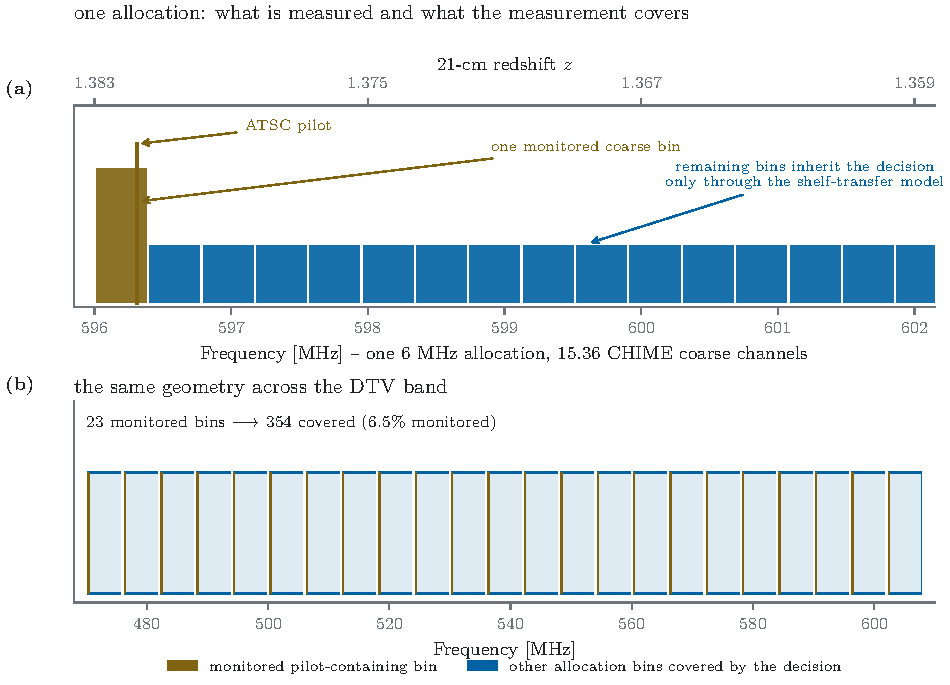
\includegraphics[width=0.98\linewidth]{figs/fig_bao_footprint.pdf}
\caption[The footprint geometry]{The footprint geometry. (a) One ATSC allocation at CHIME's coarse raster: the pilot-containing bin read by the detector against the remaining bins covered by the same decision. The different heights distinguish the monitored bin from the shelf-covered bins and are schematic, not measured power. Flatness across the received allocation is a transfer assumption to be tested, not a consequence of monitoring one pilot bin. (b) The same geometry across the DTV band under the disposition's inclusive edge-bin convention: 23 monitored bins carrying decisions for 354 CHIME coarse channels.}
\label{fig:tolerance:footprint}
\end{figure}

Three properties make the transfer from the monitored bin to the rest legitimate rather than merely convenient, and the third is an assumption rather than a result.

\textit{The screening template is flat in spectral density.} The pilot measurement is converted to a nominal payload spectral density using Eq.~\eqref{eq:shelfproxy}; the forecast then assigns that density to the payload-bearing coarse channels.  This makes $r$ a per-bin quantity and gives a clear, reproducible masking footprint.  It does \emph{not} prove that the received shelf is flat: transmitter filtering, channel response, and frequency-selective multipath can change both level and shape across 6~MHz.  Uniform application can therefore over-mask a cleaner bin or under-protect a locally enhanced one.  The simultaneous across-allocation measurement described below is the gate that decides which occurs.

\textit{The monitored bin is the one bin worth spending.} Two properties make the pilot-containing coarse channel a natural standing excision candidate in the present model. First, it is the most contaminated: the pilot carries $P_{\text{shelf}}/13.4$ while one coarse channel receives $P_{\text{shelf}}/13.8$ of the payload, so the pilot line is within $3\%$ of exactly as strong as the shelf in one bin --- a coincidence of the broadcast standard against this receiver's raster --- and the bin containing it holds $3.1$~dB more DTV power than its neighbors. Second, and decisively, the delay filter cannot help it. The shelf's suppression under a delay cut (the $3.6$--$11.4$~dB of Section~\ref{sec:tolerance:chain}) exists \emph{because} the shelf is band-limited to $B_N = 5.38$~MHz, whose delay-space envelope has its first null at $1/B_N = 186$~ns and therefore concentrates below any cut near that scale; a pilot confined to a single coarse channel is a near-delta in frequency, hence uniform in delay, and leaks into every delay the analysis retains --- including the acoustic ones. Because a narrow line is not preferentially confined to the low-delay region removed from a smooth shelf, the current analysis treats the pilot-containing coarse channel as a standing frequency excision; that treatment should be verified against the actual channelized response used by the BAO pipeline. That excision is the method's standing cost --- one bin per allocation, $6.5\%$ of the DTV band --- and it is levied on the bin the analysis would have had to discard anyway.

\textit{The transfer itself is an assumption, and the products in hand cannot close it.} Equation~\eqref{eq:shelfproxy} is a nominal transmitter model derived from the standard's pilot bias and equiprobable payload symbols; the received ratio scatters about it through frequency-selective propagation across $6$~MHz, since nothing requires a multipath null to fall on the pilot and on the far edge of the shelf alike. The survey products record only the pilot's own coarse channel --- their integrated spectra are the $16384$-point fine structure \emph{within} that one channel, not a view across the allocation --- so nothing in the present data verifies that the shelf is where the proxy says it is. Closing this requires the deployment to record, for a subset of frames, integrated spectra in coarse channels distributed across the allocation, masked and unmasked, and to confirm that the shelf removal in those channels tracks the level inferred from the pilot. That measurement is the direct test of the premise the method is named for. It is specified here as a requirement on the implementation, and it is not attempted from the survey archive, whose per-channel products were never built to carry it.

The leverage and the assumption are the same statement seen from two sides. A method that measured contamination in the bins it protects would need no proxy and would offer no leverage; the pilot buys a factor of $15$ in coverage at the price of one inference, and the reach of every verdict below is ultimately bounded by how well that inference is checked. What follows prices the decision under that transfer model.  Results are labelled conditional until its measured distribution is propagated through the forecast.

\section{The Cost Side: Masking Alone}
\label{sec:tolerance:cost}

A per-frame mask enters radiometric cost through the masked fraction $f$ and a \emph{stochastic equivalent-variance ratio} $r_{\rm var}$ for contamination surviving in the kept frames.  Discarding frames scales the effective integration as $t \to t(1-f)$; a noise-like residual scales the variance as $\sigma^2 \to \sigma^2(1+r_{\rm var})$.  The integration time to reach a fixed statistical-error target therefore obeys
\begin{equation}
\label{eq:tolerance:teff}
\frac{T(f, r_{\rm var})}{T_{\text{clean}}} = \frac{1 + r_{\rm var}}{1 - f}.
\end{equation}
This is the statistical-cost functional.  A coherent residual systematic is not an added variance and is carried separately as $r_{\rm sys}$ through the Fisher-bias calculation.  The present screening analysis derives one scalar proxy $r_{\rm proxy}$ and, pending direct visibility calibration, applies it to both roles: $r_{\rm var}=r_{\rm sys}=r_{\rm proxy}$.  That equality is a declared modelling closure, not an identity.  The two failure directions remain visible: $f\to1$ consumes the data, while either residual component can make the retained data unusable.

Within a forecast redshift bin the per-channel weights $w_c = (1 - f_c)/(1 + r_{{\rm var},c})$ must be reduced to a band average, and the reduction is not unique --- it encodes a physical assumption about how surviving frames populate the modes the analysis measures:
\begin{equation}
\label{eq:tolerance:wbar}
\bar{w}_{\text{inv}} = \langle w \rangle_B, \qquad
\bar{w}_{\text{four}} = \left\langle w^{-1} \right\rangle_B^{-1},
\end{equation}
where $\langle\cdot\rangle_B$ is the bandwidth-weighted mean over the bin. The inverse-variance form $\bar{w}_{\text{inv}}$ holds when kept frames are distributed so that every mode sees the average depth --- the correct convention for masking that is uncorrelated with sidereal time. The harmonic form $\bar{w}_{\text{four}}$ holds when radial Fourier modes require simultaneous coverage across the bin, so the thinnest slice throttles every mode that crosses it; it is the pessimistic convention, and a single near-fully-masked channel drags the entire bin ($w \to 0$ forces $\bar{w}_{\text{four}} \to 0$ while $\bar{w}_{\text{inv}}$ barely moves). Both are implemented; the two conventions move the band-level forecast by well under a percent, because the per-channel rates are either mild (most channels) or so severe that the channel is excised outright and leaves the average entirely. Excision is priced separately and differently: an excised channel is removed from the bin's \emph{volume} (Fisher information scales linearly with surviving bandwidth), never from its noise, because no integration time recovers a band that is not observed.


\begin{figure}[t]
\centering
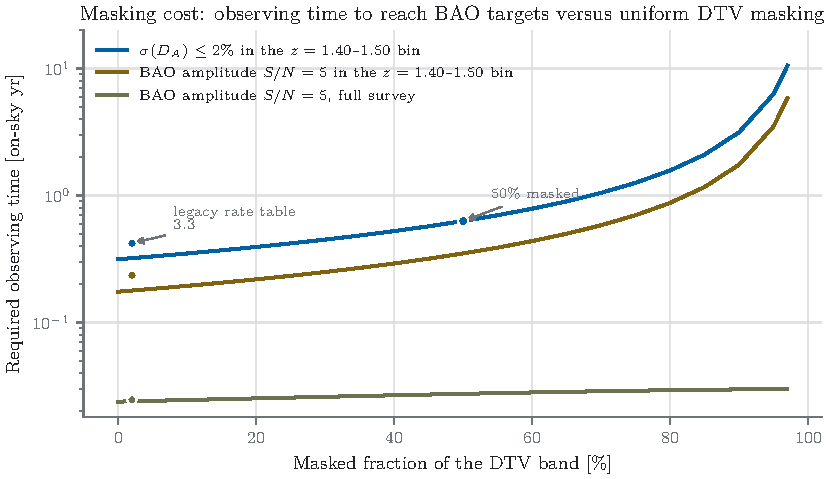
\includegraphics[width=0.98\linewidth]{figs/fig_bao_time_vs_masking.pdf}
\caption[Masking-cost curve]{Integration time to fixed BAO targets versus masked fraction in the DTV band, at $r = 0$ (masking cost only, Eq.~\eqref{eq:tolerance:teff} with the band averaging of Eq.~\eqref{eq:tolerance:wbar}). The curve is the algebraic cost map; the per-channel inputs that place each policy on it are the masked fractions of Table~\ref{tab:tolerance:eta}, and what a mask \emph{buys} still requires the residual chain of Section~\ref{sec:tolerance:chain}.
\stub{v5 archive rerun}{Regenerate without the historical annotations; mark the band-level masked fraction at the selected per-channel operating points, with the flag rate shown only as an occupancy reference.}}
\label{fig:tolerance:time}
\end{figure}

Equation~\eqref{eq:tolerance:teff} with $r_{\rm var} = 0$ prices only the cost of masking, and on that accounting the mask looks nearly free --- which is precisely why cost-only accounting is insufficient. The benefit side requires knowing what contamination survives in the frames each policy keeps, and that is a measurement problem the next section turns into a four-term chain.

\section{The Benefit Side: the Contamination-Residual Chain}
\label{sec:tolerance:chain}

The survey does not directly observe the final visibility-domain contamination residual.  It observes a scalar pilot-power proxy, and the residual chain propagates that proxy through a timescale model.  Define
\begin{align}
\label{eq:tolerance:chain}
p_{\rm kept} &\equiv 10^{(S_{\text{kept}}-S_{\text{delay}})/10},\\
r_{\rm proxy} &\equiv p_{\rm kept}
  \left(\rho_{\text{intra}} n_{\text{coh,intra}}
       +\rho_{\text{fast}} n_{\text{coh,fast}}\right),\\
n_{\text{coh,intra}} &\equiv
  \frac{\min(\tau_c,T_{\text{sid}})}{T_{\text{frame}}},
  \qquad
n_{\text{coh,fast}}\equiv1.
\end{align}
Here $S_{\text{kept}}$ is the kept-frame shelf level in dB relative to per-frame system noise under the pilot-to-shelf model; $S_{\text{delay}}$ is any delay-filter credit booked on both sides of the calculation; $\rho_{\text{intra}}$ and $\rho_{\text{fast}}$ are normalized second-moment shares of the scalar proxy defined below; and $\tau_c$ is the intra-day correlation-time outcome.  The numerical tables use $r_{\rm proxy}$ as a screening envelope.  The physically distinct forecast inputs are
\begin{equation}
  r_{\rm var}=g_{\rm var}r_{\rm proxy},
  \qquad
  r_{\rm sys}=g_{\rm sys}r_{\rm proxy},
  \label{eq:tolerance:transfer}
\end{equation}
where $g_{\rm var}$ and $g_{\rm sys}$ map the scalar proxy to stochastic covariance and coherent visibility bias.  Those transfer coefficients are not measured by the present pilot-only products; the screening results below set both to unity and are conditional on that normalization.  Direct complex-visibility measurements are required to replace it.

\begin{figure}[t]
\centering
\resizebox{\linewidth}{!}{% Editable source for Figure \ref{fig:tolerance:chainaudit}: the residual chain and its evidence boundary.
\begin{tikzpicture}[font=\small, node distance=4mm and 5mm,
  st/.style={draw, rounded corners=2pt, align=center, inner sep=3.5pt, minimum height=19mm, text width=#1, line width=0.75pt},
  ex/.style={st=#1, fill=ppMeasured!8, draw=ppMeasured!90!black},
  md/.style={st=#1, fill=ppModel!10, draw=ppModel!90!black},
  cd/.style={st=#1, fill=ppConditional!10, draw=ppConditional!90!black},
  ctx/.style={st=#1, fill=black!2, draw=ppPending!90!black},
  arr/.style={-{Stealth[length=1.8mm]}, thick, ppPending!85!black}]
\node[ex=26mm] (a) {\textbf{pilot statistic}\\measured per frame\\$e = F/\mu_0 - 1$};
\node[md=26mm, right=of a] (b) {\textbf{pilot $\to$ shelf}\\$\times\,336/25$ ($+11.3$~dB); local shape $g$; propagation};
\node[ex=26mm, right=of b] (c) {\textbf{kept-frame floor}\\measured on the era, or refused};
\node[ex=26mm, right=of c] (d) {\textbf{day variation}\\intra/inter-day shares; $\tau_c$: measured, bound, refused};
\node[md=26mm, right=of d] (e) {\textbf{visibility residual}\\proxy $\to$ $(r_{\rm var}, r_{\rm sys})$ transfer};
\node[cd=26mm, right=of e] (f) {\textbf{$P(k)$ bias}\\Fisher forecast against $r_{\rm tol}$};
\foreach \p/\q in {a/b,b/c,c/d,d/e,e/f} \draw[arr] (\p) -- (\q);
\node[ctx=44mm, below=8mm of c, xshift=12mm] (rv) {$r_{\rm var}$ adds to the covariance: averages with the declared coherence model};
\node[ctx=44mm, right=8mm of rv] (rs) {$r_{\rm sys}$ enters a signed residual template: parameter-bias calculation};
\draw[thick, ppPending!85!black] (e.south) -- ++(0,-3.5mm) coordinate (j);
\draw[thick, ppPending!85!black] (j -| rv.north) -- (j -| rs.north);
\draw[arr] (j -| rv.north) -- (rv.north); \draw[arr] (j -| rs.north) -- (rs.north);
\node[font=\scriptsize, text=ppModel!95!black, align=center, above=5mm of c, text width=110mm] {blue: measured on the archive per channel and era \quad gold: model gates the archive cannot close alone \quad green: forecast};
\node[draw=ppModel!90!black, dashed, rounded corners=2pt, fill=ppModel!5, align=center, font=\scriptsize, text width=140mm, inner sep=3pt, below=6mm of rv, xshift=25mm]
  {closing tests that turn the gold gates into measurements: simultaneous full-allocation spectra (pilot $\to$ shelf); contaminated complex visibilities before and after the sidereal filter (proxy $\to$ visibility); an empirical residual template through the combined-bin estimator};
\end{tikzpicture}
}
\caption[Residual-chain evidence audit]{The residual chain and its evidence
boundary.  Pilot power, archive timescale structure, and correlation-time
outcomes are scalar measurements.  Across-allocation transfer and the mapping to
complex visibility covariance and bias are separate, load-bearing calibrations.
The current numerical forecast closes those arrows with a stated unity transfer;
it does not turn them into measured equalities.}
\label{fig:tolerance:chainaudit}
\end{figure}

\subsection*{The delay filter, and the one assumption this section makes}

Foreground removal in 21\,cm analysis exploits spectral smoothness: astrophysical foregrounds are confined to low delay $\tau$ (the Fourier dual of frequency), while cosmological structure extends to higher delay through the mapping
\begin{equation}
\label{eq:tolerance:kpar}
k_\parallel = \frac{2\pi\, \nu_{21}\, H_0 E(z)}{c\, (1+z)^2}\, \tau
\end{equation}
\cite{amiri2023detection}. A delay cut $\tau_{\text{cut}}$ therefore removes DTV power --- which, arriving through a $\sim$few-$\mu$s multipath spread but dominated by the direct path, is itself spectrally smooth over the $390$~kHz coarse channel --- along with the foregrounds. The published analyses cut at $\tau_{\text{cut}} = 200$~ns, which suppresses the coarse-channel-confined shelf by $11.4$~dB; but the same cut removes the low-$k_\parallel$ modes carrying the acoustic feature, and the hybrid foreground-removal demonstration states directly that the standard filter excludes any sensitivity to BAO \cite{chime2024hybrid}. A BAO analysis in this band must therefore \emph{relax} the filter: preserving the second acoustic peak ($\tau \approx 104$~ns at these redshifts, via Eq.~\eqref{eq:tolerance:kpar}) admits a cut buying $8.2$~dB of shelf suppression; preserving the first peak ($\tau \approx 56$~ns) buys only $3.6$~dB. This is the structural irony on which the whole problem rests: \emph{the analysis choice that makes BAO measurable is the same choice that re-admits DTV}, so the two problems --- foreground filtering and RFI masking --- cannot be solved independently.

Under the Overview-forecast convention of Section~\ref{sec:tolerance:scope} --- no foreground removal modelled --- however, the correct value to use for $S_{\text{delay}}$ is \emph{zero}, and that is what every number below adopts. The forecast carries no foreground removal, so the chain may not bank suppression from a filter the forecast does not model; the range $3.6$--$11.4$~dB is retained not as an assumption but as a bound on the help that would become available if the filter were carried on both sides of the calculation. Setting it to zero is conservative with respect to this one suppression term --- it makes every scalar-chain residual $2.3\times$ larger than the first-peak value would.  It does not make the chain assumption-free: the pilot-to-allocation transfer, scalar-to-visibility transfer, and residual template remain modelling choices.  Any filter carried self-consistently in both the residual and Fisher models can reduce the smooth component, but the effect on the full visibility residual must be measured rather than inferred from the scalar shelf alone.

\medskip
\noindent\textbf{\textit{A note on the deployed cut, and the era it does not describe.}} One consequence of the trade above deserves to be stated on its own, carefully, because it is prospective rather than retrospective. Nothing in it identifies an error in any published CHIME result: no released analysis relies on the low-$k_\parallel$ region, and for the analyses actually published the $200$~ns cut is the appropriate choice. The observation is about what that choice has quietly done to everyone's \emph{experience} of the interference environment. Every characterization of RFI cleanliness earned to date --- inspected maps, flagger performance, residual levels judged acceptable --- has been earned in data filtered at $200$~ns, which is to say with $11.4$~dB of incidental DTV suppression silently included. A BAO analysis must hand back $3.2$--$7.8$~dB of that discount, so the DTV residual a BAO pipeline will face is four to six times the one present experience exhibits --- and it arrives at exactly the moment the tightest tolerances of Section~\ref{sec:tolerance:fisher} come into force. An assessment of ``whether RFI is under control,'' calibrated on the current pipeline, therefore does not transfer to the BAO configuration: it understates the problem by precisely the suppression that must be traded away to make BAO measurable at all. In the most cautious reading this is bookkeeping --- a reminder that cleanliness observed in today's maps is a property of today's filter, not of the band. In the least cautious reading it flags a risk worth naming: that the band could be judged manageable from experience gathered in the one configuration that will not be used to measure BAO. The present work takes no position between those readings --- there is not enough information to take one --- but the masking infrastructure it builds is aimed, deliberately, at the harsher configuration: the one CHIME has not yet operated in, and the only one in which the ruler can be read.

\subsection*{The sidereal filter: a scalar-proxy decomposition}

The analysis subtracts a per-sidereal-day mean from each complex visibility
\cite{amiri2023detection}.  The present archive does not contain the corresponding
baseline-resolved complex visibilities; it contains a dimensionless scalar shelf
power ratio.  The decomposition below is therefore a model of the proxy's
timescale structure, not a direct measurement of the visibility attenuation.
Write
\begin{equation}
\label{eq:tolerance:anova}
p_{dui}=\mu+a_d+b_{du}+\varepsilon_{dui},
\end{equation}
for frame $i$, acquisition $u$, and sidereal day $d$, with centered random
effects $a_d$, $b_{du}$, and $\varepsilon_{dui}$.  Define the proxy second-moment
normalization
\begin{equation}
 Q_p=\mu^2+\operatorname{Var}(a)+\operatorname{Var}(b)
       +\operatorname{Var}(\varepsilon),
\end{equation}
and
\begin{equation}
 \varphi_{\rm intra}=\frac{\operatorname{Var}(b)}{Q_p},
 \qquad
 \varphi_{\rm fast}=\frac{\operatorname{Var}(\varepsilon)}{Q_p}.
\end{equation}
This construction is dimensionally consistent: every term in $Q_p$ is a squared
power-ratio fluctuation.  It locates the scalar proxy's slow and fast variability
relative to the sidereal-day boundary.  It does not establish that the same
fractions survive a linear operation on complex baseline visibilities, because
the pilot-power product has discarded cross-feed phase and baseline structure.

The current screening calculation treats $\mu^2+\operatorname{Var}(a)$ as the
proxy share removed by the daily-mean operation and the remaining two shares as
survivors.  On one measured channel this assigns approximately \rerun{99\%} of the proxy's second
moment to the removed side, corresponding to a \rerun{20-dB} scalar-chain
suppression.  That number is useful for prioritizing measurements, but it is not
a measured visibility-domain suppression.  The closing test records contaminated
complex visibilities before and after the actual per-day operator and estimates
$g_{\rm var}$ and $g_{\rm sys}$ by baseline, frequency, and epoch.  The operator
is an explicit analysis choice applied to data; the transit geometry also makes
a truly static telescope-frame mode difficult to distinguish, but that fact does
not by itself prove the scalar attenuation used here.

\subsection*{Coherence: how the survivors average}

Thermal-noise variance in an integrated estimate falls approximately as $1/N_{\text{frames}}$.  The scalar screen treats each slow component as a rectangular coherent block and therefore assigns the amplification $n_{\text{coh,intra}}=\tau_c/T_{\rm frame}$ of Eq.~\eqref{eq:tolerance:chain}; the explicitly defined fast factor is $n_{\text{coh,fast}}=1$.  That ratio is exact for the declared block model, not for an arbitrary autocorrelation function.  In general the variance of an average depends on the weighted integral of the autocorrelation \cite{bartlett1946,geyer1992}; for a densely sampled exponential correlation the large-$N$ factor approaches roughly $2\tau_c/T_{\rm frame}$ rather than $\tau_c/T_{\rm frame}$.  The sidereal-day cap prevents the scalar model from assigning unlimited coherence to structure that the per-day operator is intended to remove.  It is a bookkeeping convention, not proof that every longer-lived visibility contaminant is exactly removed.  Keeping the slow and fast terms separate avoids applying the slow component's amplification to the noise-like sub-acquisition fluctuations.

The archive supplies a same-day structure-function timescale for the shelf: the variance between same-day acquisition pairs is evaluated as a function of lag, the characteristic decorrelation lag is read from the approach to the plateau, and uncertainties come from a bootstrap over whole sidereal-day blocks (resampling frames would fabricate independence the data does not have) \cite{kunsch1989}.  That plateau lag is not, in general, identical to the integrated autocorrelation time that determines an effective sample count.  The present scalar chain uses it as a persistence descriptor inside the rectangular-block screen and therefore reports measured values or bounds with this modelling qualification; contiguous data are required to integrate the autocorrelation function directly.  Sparse cadence and finite duration can also create apparent structure-function breaks, so an operational use requires cadence-matched coverage tests in addition to the day bootstrap \cite{emmanoulopoulos2010}. The estimator refuses rather than extrapolates: a channel whose apparent $\tau_c$ moves by more than a factor-of-stability threshold across trim percentiles is declared \emph{episodic} --- the shelf is not a stationary process with one correlation time --- and the chain falls back to the sidereal-day cap, reported as a bound rather than a measurement. The screening model treats surviving intra-day proxy fluctuations as independent across days.  Civil-time transmitter schedules precess through sidereal time by about 3.93~min per solar day, and meteorological propagation is not naturally locked to the sky; these facts motivate the assumption but do not guarantee it.  A sidereal-coherent component is therefore one of the alternative residual templates and direct visibility tests required below.

\section{The Decision: Four Policies, One Ordering}
\label{sec:tolerance:policy}

A survey holding a DTV-contaminated channel has exactly four options, and the detector must be priced against all of them, not against a straw man: \emph{keep} everything ($f = 0$); \emph{excise} the channel ($f = 1$; infinite time-to-measurement in band, volume loss at survey level); flag with the \emph{incumbent} methods already in the pipeline (Section~\ref{sec:tolerance:incumbent}); or flag on the \emph{pilot}. Each policy supplies a masked fraction $f$ and a scalar residual proxy $r_{\rm proxy}$.  Equation~\eqref{eq:tolerance:transfer} then maps that proxy to the two quantities the forecast actually needs: $r_{\rm var}$ for statistical cost and $r_{\rm sys}$ for coherent bias.  The tables of this chapter use the unity-transfer screening closure, so their single reported residual should be read as $r_{\rm proxy}$ rather than as a direct visibility measurement.

At the \emph{frame} stage --- kept-frame mean shelf power, no downstream chain --- keeping everything wins on most channels, and it is worth stating this plainly rather than hiding it: the raw scalar shelf ratios are small (on the superseded products, \rerun{$r_{\rm proxy} = 4\times10^{-4}$ to $0.085$} on the channels first analysed).  Were those ratios already calibrated as purely stochastic visibility variance, integrating through them would be cheaper than cutting around them.  The qualification matters: frame-level scalar power is not yet the final visibility residual.

The scalar coherence model is what overturns the frame-level ordering, and the timescale measurement is where it happens.  A channel whose structure function yields $\tau_c$ of tens of minutes carries $n_{\mathrm{coh,intra}}$ of order $10^4$--$10^5$; under the proxy decomposition and unity-transfer closure a modest sub-noise on-air shelf then becomes an $r_{\rm proxy}$ of order tens under the keep policy, whereas any mask that removes the detectable-pilot population spends $1/(1-f)$ before a retained-frame residual is charged.  The defensible conclusion is narrower and still useful: a sub-noise shelf can become survey-limiting when its measured timescale is long, and $\tau_c$ is a load-bearing discriminator that must be carried into the direct visibility calibration.

The opposite face must be reported with equal prominence.  A channel whose flag rate is near unity --- the transmitter present in nearly every archived frame --- is one on which any mask that removes the detectable-pilot population costs at least $1/(1-f)$, two orders of magnitude at $f = 0.99$, regardless of how clean the kept frames are, because on an always-on channel that population is almost every valid frame.  The keep-policy scalar chain on such a channel is itself only a bound when $\tau_c$ is refused and replaced by the sidereal cap.  Thus the archive does not by itself identify a favorable policy; it identifies an operating-point problem and, where $\tau_c$ is refused, a missing cadence measurement.  The role of Eq.~\eqref{eq:tolerance:chain} is to convert each candidate threshold $\eta$ into $(f,r_{\rm proxy})$, after which the calibrated transfers, statistical cost, and bias constraint can be evaluated separately.  A runtime threshold is selected only after that full, held-out calculation.

\section{The Incumbent Comparison: Why a Reference Beats a Baseline}
\label{sec:tolerance:incumbent}

The four-policy ordering requires measuring the incumbents, not asserting them. Two families cover what 21\,cm pipelines commonly use: outlier rejection on integrated power at a few-second cadence with a MAD-scaled threshold ($\text{median}+1.8\times\text{MAD}$ in the published CHIME configuration \cite{amiri2023detection}), and spectral kurtosis \cite{nita2010sk}, which tests departures from a calibrated Gaussian-like power distribution.  A high-duty-cycle transmitter can contaminate the reference population of a block statistic: the median then follows the occupied state and a steady excess becomes difficult for a MAD cut to distinguish.  Spectral kurtosis has a different limitation.  Its expectation is power-invariant for an ideal stationary Gaussian process \cite{nita2010sk}, so a stationary power excess whose filtered, coded 8-VSB samples remain close to the calibrated null shape can evade it.  A real 8-VSB waveform is synchronized, filtered, coded, and quantized, and is therefore not mathematically identical to a Gaussian process; the limitation is empirical and model-dependent, not a theorem that every DTV shelf is exactly the SK null.  The pilot statistic supplies an external frequency reference and therefore does not estimate its line location from the occupied power baseline.  Synthetic tests and the common-frame comparison of Table~\ref{tab:tolerance:flaggers} quantify the advantage for the present cohort without claiming universal dominance over every cyclostationary or decoding-based detector.

\begin{table}[t]
\centering
\caption[Every flagger on the same frames]{Every flagger on the same frames (three-channel example from the superseded products; values in blue are to be regenerated and extended to all 23 channels on their current eras): shelf power removed from the kept population (dB), with the masked fraction each spends to do it. Measured within acquisitions on the survey products; the per-frame shelf is the pilot matched filter's own measurement, common to all rows (frames with no detection are assigned the sensitivity floor, a conservative choice that penalizes all flaggers equally, including the pilot proxy). Duty cycle is the fraction of valid frames carrying a positive pilot excess.}
\label{tab:tolerance:flaggers}
\begin{tabular}{lccc ccc}
\toprule
 & \multicolumn{3}{c}{shelf removed (dB)} & \multicolumn{3}{c}{masked fraction $f$} \\
\cmidrule(lr){2-4}\cmidrule(lr){5-7}
 & ch\,34 & ch\,35 & ch\,36 & ch\,34 & ch\,35 & ch\,36 \\
\midrule
duty cycle & \rerun{$0.991$} & \rerun{$0.837$} & \rerun{$0.999$} & & & \\
MAD $1.8\times$ (per acquisition) & \rerun{$0.09$} & \rerun{$0.01$} & \rerun{$0.02$} & \rerun{$0.067$} & \rerun{$0.056$} & \rerun{$0.063$} \\
spectral kurtosis, $3\sigma$ & \rerun{$6.40$} & \rerun{$0.22$} & \rerun{$8.73$} & \rerun{$0.331$} & \rerun{$0.203$} & \rerun{$0.395$} \\
pilot proxy, survey flag as stand-in & \rerun{$18.98$} & \rerun{$63.54$} & \rerun{$35.96$} & \rerun{$0.984$} & \rerun{$0.826$} & \rerun{$0.999$} \\
\bottomrule
\end{tabular}
\stub{v5 archive rerun}{Regenerate as a compact survey summary --- median and range of each flagger's suppression and masked fraction across the 23 current eras, with the pilot proxy at its selected $(\rho^\star,\eta^\star)$ as the row that matters --- and put the per-channel values in the Appendix~\ref{app:archive-diagnostics} ledger rather than a 23-row expansion here.}
\end{table}

Three caveats keep this table honest. First, the incumbents' blocks are confined within single acquisitions --- the survey holds a median of a few frames per event, spaced hours apart over \rerun{7.6 years}, and any block statistic spanning those gaps measures the archive's sampling pattern, not the sky --- which caps them at \rerun{$1.38$~s} and means \emph{the published few-second flagging cadence cannot be reproduced on this dataset at all}; the contiguous-scan campaign exists in large part to close exactly this gap. Second, the SK null is calibrated per channel so its median block sits at unity, handing the incumbent the best normalization available, tuned on the very data it is tested against --- a courtesy the pilot proxy does not receive. Third, where the shelf \emph{is} intermittent (\rerun{channels 34 and 36} carry episodic structure), SK does real work --- \rerun{$6.4$ and $8.7$~dB} --- and the comparison narrows honestly: the incumbent regime is bursty contamination, the pilot regime is steady contamination, and the DTV band is predominantly the latter. Real work, however, is not the same as sufficient work. Carried through the residual chain and compared against the tolerance evaluated in Section~\ref{sec:tolerance:fisher}, SK's several decibels leave a residual four orders of magnitude above what the growth-rate measurement can absorb; the dB column understates the gap because it is measured against the raw shelf rather than against what the science requires.

The deeper asymmetry, however, is not the dB column. Every quantity in Eq.~\eqref{eq:tolerance:chain} --- the kept-frame anchor $S_{\text{kept}}$, the timescale split, $\tau_c$ itself --- exists because the matched filter measures a per-frame shelf level through the proxy relation. An energy-threshold flagger emits a bit; the pilot proxy emits a \emph{measurement}. Even on a channel where the optimal policy turns out to be ``do not mask'' or ``excise,'' that verdict is only computable because the contamination was measured, which is why the detector's contribution survives its own negative verdicts: the alternative to the pilot proxy is not a cheaper flagger, it is not knowing $r$.

\section{Propagation to Cosmological Parameters}
\label{sec:tolerance:fisher}

The statistical and systematic residuals enter different parts of the forecast.  Masking scales the thermal covariance through $\bar w^{-1}$ (Eq.~\eqref{eq:tolerance:wbar}), and a calibrated stochastic residual adds $r_{\rm var}C_N$ to that covariance.  A coherent residual instead enters through a unit noise-shaped template whose signed amplitude is $A$:
\begin{equation}
  C_{\rm tot}(k,\mu;z;A)
  = C_{\rm base}(k,\mu;z) + A\,C_N(k,\mu;z;T^\ast),
  \label{eq:tolerance:template}
\end{equation}
where $C_N(T^\ast)$ is frozen at the target integration used to define the tolerance and $C_{\rm base}$ contains the otherwise modelled covariance.  This is a \emph{thermal-noise-shaped contamination template} used for screening, not a claim that DTV residuals physically share the full $k$, $\mu$, redshift, baseline, or sidereal structure of thermal noise.  The amplitude $A$ is appended to the Fisher matrix through $\partial\ln C_{\rm tot}/\partial A=C_N/C_{\rm tot}$.  Let $\boldsymbol\theta$ denote the fitted cosmological and nuisance parameters other than $A$, let $A_{\rm fixed}$ be the amplitude imposed in the fit, and define the signed mismatch $\Delta A\equiv A_{\rm true}-A_{\rm fixed}$.  Under the present scalar closure, $|\Delta A|=r_{\rm sys}$; the residual is not multiplied by $r_{\rm sys}$ a second time inside the unit template.  To first order, fixing the wrong amplitude gives
\begin{equation}
\label{eq:tolerance:bias}
\Delta\boldsymbol\theta
 = F_{\theta\theta}^{-1}\,\boldsymbol F_{\theta A}\,\Delta A,
\qquad
\Delta\boldsymbol\theta\equiv
\boldsymbol\theta_{\rm fit}-\boldsymbol\theta_{\rm true},
\end{equation}
where $F_{\theta\theta}$ is the block for the parameters that remain free in the fit and $\boldsymbol F_{\theta A}$ is its cross block with the omitted amplitude.  Thus the inverse is not the inverse of the augmented Fisher matrix in which $A$ is allowed to float: that marginalization answers a different question.  Reversing the definition of $\Delta A$ reverses the displayed sign, while every tolerance below uses $|\Delta\boldsymbol\theta|$ and is sign-invariant.  The statistical cost and coherent bias therefore remain distinct even when the present screening closure sets their scalar normalizations equal.

\subsection*{Residual-shape and time-scaling gates}

The noise-shaped template is one member of a required sensitivity bank, not the
final physical model.  The model-only bank builder now supplies four named,
unit-amplitude families that the available RadioFisher callable can represent:
noise-shaped; a Gaussian envelope in low $|k_\parallel|$; a declared linear
wedge with a Gaussian roll-off; and a shell localized in $|k|$.  The family,
normalization, parameters, and authenticated source identities travel with the
bank.  The callable has no observing-frequency, baseline-vector, sidereal-time,
or measured-visibility coordinate, so a frequency-localized,
sidereal-coherent, or empirical visibility template cannot be created honestly
from the forecast repository alone.  Those remaining families require the
direct visibility products, which also supply the transfer coefficients of
Eq.~\eqref{eq:tolerance:transfer}.  A channel retains its class only if the class is
stable across the analytic and empirical templates justified by those data;
otherwise it is labelled template-sensitive.

Time scaling must be tied to the definition of the residual.  The forecast now
implements both conventions as named families.  In
\texttt{noise\_normalized\_at\_each\_time}, the reported amplitude is
$r(t)=P_{\rm res}(t)/P_N(t)$ and the unit template follows the contemporaneous
thermal power; this is the convention of the existing convergence figure.  In
\texttt{fixed\_physical\_at\_reference\_time}, the reported amplitude is
$r_{\rm ref}=P_{\rm res}/P_N(t_{\rm ref})$, and the unit-bank response receives
the explicit multiplier $t/t_{\rm ref}$.  The two families agree exactly at
$t_{\rm ref}$ and answer different questions away from it.  The response-bank
amplitude is applied once through $\Delta A$; multiplying the template by an
external $r_{\rm sys}$ as well would double-count the contaminant.  A bounded
three-time evidence run verifies the reference-time equality and exact
$t/t_{\rm ref}$ multipliers while retaining lower, central, upper, condition,
eigenmode, sign, movement, and refusal records for every requested target.

The paper default is the per-bin Appendix-A estimator with the noise-normalized time family. Three numerical gates are also part of the decision record rather than hidden solver constants: modes beyond condition number $10^{12}$ are unresolved, null-space projections are screened at $\sqrt{\epsilon_{64}}=1.4901161\times10^{-8}$, and redshift slices with retained volume fraction at or below $10^{-6}$ are skipped. These follow standard conditioning practice \cite{higham2002}, but the exact values are provisional sensitivity choices: the recorded probes are $10^{10}$--$10^{14}$ for the condition limit, machine epsilon through $10^{-6}$ for the null-space cutoff, and zero through $10^{-4}$ for the volume floor. Changing any of them changes the tolerance calculation and therefore requires a new decision digest.

The bias tolerance
\begin{equation}
\label{eq:tolerance:rtol}
r_{\text{tol}}(T^\ast) = \max \left\{ r_{\rm sys} : \left| \Delta\alpha(r_{\rm sys}) \right| \le \zeta\, \sigma_\alpha(T^\ast) \right\}
\end{equation}
--- the largest residual whose induced bias stays below a stated fraction $\zeta$ of the statistical error at the survey's target integration $T^\ast$ --- is then the number that closes the loop of this entire dissertation.  Upstream preparation converts the latest-era frame measurements into complete, calibrated residual-score histograms indexed by $\rho$.  The exact bridge from schema-v5 integer fine powers to the all-rank Q16 score arrays is implemented; constructing an authorized science histogram still awaits accepted archive products and the declared correlation, transfer, and stability evidence.  The threshold selector receives that mapping and $r_{\text{tol}}$, derives $(f,r_{\rm var},r_{\rm sys})$ by cumulative bin sums, and returns $(\rho,\eta)$.  Equation~\eqref{eq:tolerance:teff} then prices that result against keep, excise, and incumbent.  Era boundaries, valid-row filtering, floors, correlation treatment, and transfer calibration determine the prepared family; stability and evidence gates determine whether that family is authorized for selection. None is a separate selector input.

\subsection*{Objective and target time}

Three parameters appear in this chapter and one of them decides. The
\emph{primary objective} for every per-channel decision is the pair of acoustic
dilations $(\alpha_\perp, \alpha_\parallel)$ of the channel's own redshift bin
on the operable, no-delay-filter tier --- the ruler alone, the measurement a
mask-only analysis can make. The single primary criterion is $R_{\rm dil} = r_{\rm sys}/\min(r_{\perp}, r_{\parallel}) \le 1$,
evaluated on the bin's own tolerances and reported with both components.
The growth rate $f\sigma_8$ is the \emph{binding
secondary}: it is reported at the same point for every channel, it is ten to
twenty-five times more delicate, and it is the objective of the filtered
worlds of Section~\ref{sec:tolerance:worlds}. $D_V$ is the summary of the
dilations that the Overview forecast quotes, not a separate objective. The
target time is fixed: $T^\ast$ is one on-sky year of integration on the
Overview-convention bank, the reference at which every tolerance in
Table~\ref{tab:tolerance:rtol} is quoted and at which the fixed-physical and
noise-normalized conventions agree by construction; the cost functional prices
departures from it.

\subsection*{The tolerance, evaluated}

Equation~\eqref{eq:tolerance:rtol} is not blocked on channel coverage: $r_{\text{tol}}$ is a property of the survey and the forecast, and only its conversion into per-channel thresholds needs the channels. Evaluating it on a Fisher bank carrying the \texttt{\_Pres} row --- built with $P_{\text{res}}=1$, so the unit template is the reference-time noise power and $|\Delta A|=r_{\rm sys}$ supplies its physical amplitude --- gives the result in Table~\ref{tab:tolerance:rtol}. Two features of it are worth more than the number.

First, \emph{the growth rate binds, not the acoustic dilations}. At $\zeta = 1$, $f\sigma_8$ tolerates $r \approx 1.5 \times 10^{-3}$ while $\alpha_\perp$ and $\alpha_\parallel$ tolerate roughly ten times more, and the ordering holds in every DTV redshift bin at every integration time. This is what should be expected on reflection: the acoustic scale is a feature \emph{position}, protected by the oscillatory signature that defines it, and a smooth additive residual displaces it only weakly; the growth rate is read off an \emph{amplitude}, which is precisely what an additive residual counterfeits. A framework that had priced only the BAO dilations would have concluded the band was ten times safer than it is.

Second, \emph{the dilations cannot be read off the grid unguarded}, and the reason is physical rather than numerical. The response $D_p(T)\equiv\partial p/\partial r_{\rm sys}$ can pass smoothly through zero as sample variance overtakes thermal noise.  Near such a crossing Eq.~\eqref{eq:tolerance:rtol} can report a spuriously large tolerance.  For each parameter $p$ and central time $T$, define $D_-=D_p(0.9T)$, $D_0=D_p(T)$, and $D_+=D_p(1.1T)$.  With a declared numerical scale $\epsilon_D$, an entry is accepted only if
\begin{equation}
\label{eq:tolerance:stability}
 |D_0|>\epsilon_D,\qquad
 \operatorname{sgn}(D_-)=\operatorname{sgn}(D_0)=\operatorname{sgn}(D_+),\qquad
 \max_{s\in\{-,+\}}\left|\frac{D_s}{D_0}-1\right|\le0.20.
\end{equation}
The release records $\epsilon_D$, the three derivatives, and the rejection reason.  On the present 19-point grid the gate refused several dilation entries and no $f\sigma_8$ entries; a 32-point grid refined through the crossings reproduced the shared Fisher matrices to all printed digits and did not change the qualitative result.  The crossings are structure, not a coarse-grid artifact.

What survives the gate is usable, and it is the second tier of the tolerance story. The stable dilation entries that remain in every DTV bin have per-bin minima of $r_{\rm tol}(\alpha_\perp) = 0.014$--$0.035$ at $\zeta = 1$ --- an order of magnitude looser than $f\sigma_8$, exactly the asymmetry Figure~\ref{fig:intro:dilation} promised. The two tiers do different work. The $f\sigma_8$ tolerance of Table~\ref{tab:tolerance:rtol} is the binding requirement for the full measurement; the stable dilation tolerance is the requirement for the \emph{ruler alone}, and it is the constraint the per-channel threshold optimization of Section~\ref{sec:tolerance:thresholds} runs on, because it is the one a no-delay-filter analysis can actually meet. The screening structure that results --- dilation-tier candidates on some channels, and growth-rate candidates only once the delay filter is booked on both sides of the calculation (Section~\ref{sec:tolerance:worlds}) --- is the two-tier headline of this section.

\begin{table}[t]
\centering
\caption[The residual tolerance by parameter and redshift bin]{The residual tolerance $r_{\text{tol}}$ of Eq.~\eqref{eq:tolerance:rtol} at this work's adopted $\zeta = 1$ systematic-budget convention, following the form of Ref.~\cite{amara2008}, per DTV redshift bin, taken over the entries that survive the stability refusal described in the text. $\alpha_\perp$ and $\alpha_\parallel$ are omitted: both are refused at several integration times in every bin, and where they survive they tolerate about ten times more than $f\sigma_8$, so they never bind. Within the current reference-time, noise-shaped template family, the tightest accepted value occurs near one on-sky year; the table reports that minimum without promoting its time dependence to a universal physical scaling law. The $f\sigma_8$ entry survives the gate at every grid point in every bin; the dilations' surviving entries are the second tier taken up in the text and in Section~\ref{sec:tolerance:thresholds}.}
\label{tab:tolerance:rtol}
\begin{tabular}{lccccccc}
\toprule
$z$ bin & $1.30$--$1.40$ & $1.40$--$1.50$ & $1.50$--$1.60$ & $1.60$--$1.70$ & $1.70$--$1.80$ & $1.80$--$1.90$ & $1.90$--$2.04$ \\
\midrule
$r_{\text{tol}}$ ($\times 10^{-3}$) & $1.50$ & $1.53$ & $1.60$ & $1.71$ & $1.81$ & $1.95$ & $1.77$ \\
\bottomrule
\end{tabular}
\end{table}

\subsection*{Closing the code-side estimator and analytic-template gates}

The per-bin, noise-shaped calculation above is no longer the only executable
forecast path.  The released completion run evaluates every one of the seven
DTV redshift bins with both the independent per-bin estimator and the joint
multi-redshift-bin Fisher estimator, for all four residual shapes supported by
the forecast callable: the noise-shaped unit template, a low-$k_\parallel$
Gaussian envelope, a linear wedge-like envelope with Gaussian roll-off, and a
shell localized in $|k|$.  Each bank carries the template family and
parameters, numerical grid, foreground and mode-cut settings, cosmology and
experiment identities, authenticated analysis-source digest, and the exact
RadioFisher source identity against which it was built.  Runtime evaluation
refuses a bank if those identities differ; file compatibility alone is not
treated as scientific compatibility.

Table~\ref{tab:tolerance:template-comparison} gives the compact result.  Its accepted
and rejected counts include the two dilation summaries as well as
$f\sigma_8$: a rejection means that the corresponding lower, central, or upper
time point failed the sign, movement, or derivative-scale gate of
Eq.~\eqref{eq:tolerance:stability}, not that a value was silently dropped.  The
growth-rate point itself is accepted at one year in all seven bins for every
analytic family.  Across bins, the independent estimator's accepted
$f\sigma_8$ tolerance spans $1.409\times10^{-3}$ to
$3.621\times10^{-3}$ over the four shapes; the joint estimator spans
$1.455\times10^{-3}$ to $3.795\times10^{-3}$.  Thus template shape changes the
permitted scalar amplitude by as much as a factor of about $2.7$ within this
model-only bank.  That spread is scientific information: it is the forecast's
sensitivity to a declared shape hypothesis, not an uncertainty distribution
over which hypothesis the real residual follows.

\begin{table}[tbp]
\centering
\caption[All-bin analytic residual-template forecast]{All-seven-DTV-bin
model-only residual-template forecast summary.  A/R is the accepted/rejected
Fisher-point count after the $\pm10\%$ integration-time stability gate.  The
per-bin column contains $7\times3=21$ one-year target points; each joint column
contains $7\times3\times3=63$ bin/time/target points.  Ranges are accepted
one-year $f\sigma_8$ residual-amplitude tolerances in contemporaneous
thermal-noise units.  The analytic-family ordering is a sensitivity envelope;
it does not revise a measured channel-policy ranking.}
\label{tab:tolerance:template-comparison}
\footnotesize
\setlength{\tabcolsep}{4pt}
\begin{tabular}{@{}lccccc@{}}
\toprule
Template & Per-bin A/R & Joint noise A/R & Joint fixed A/R & Per-bin range & Joint range \\
\midrule
Noise-shaped unit & 13/8 & 42/21 & 42/21 & 0.001503--0.001951 & 0.001620--0.002359 \\
Low-$k_\parallel$ & 15/6 & 42/21 & 42/21 & 0.002165--0.002785 & 0.002170--0.002794 \\
Wedge-like & 13/8 & 40/23 & 40/23 & 0.001409--0.001911 & 0.001455--0.002013 \\
Localized $k$ shell & 14/7 & 39/24 & 39/24 & 0.003085--0.003621 & 0.003401--0.003795 \\
\bottomrule
\end{tabular}
\end{table}

The estimator comparison is not a universal rescaling.  At one year, the
joint-to-per-bin growth-rate tolerance ratio runs from approximately unity for
the low-$k_\parallel$ family to $1.23$ for the highest-redshift noise-shaped
bin.  Figure~\ref{fig:tolerance:template-tolerances} maps the conservative value to
physical channels: when an allocation crosses a forecast-bin edge, the smaller
accepted tolerance over every bin with non-zero frequency overlap is used,
rather than an overlap-weighted value that could hide the binding side.  This
closes the code-side question of whether the earlier example bin transported
across the DTV band.  It does not close the physical question of which residual
shape applies to a given transmitter, baseline, or epoch.

\begin{figure}[tbp]
\centering
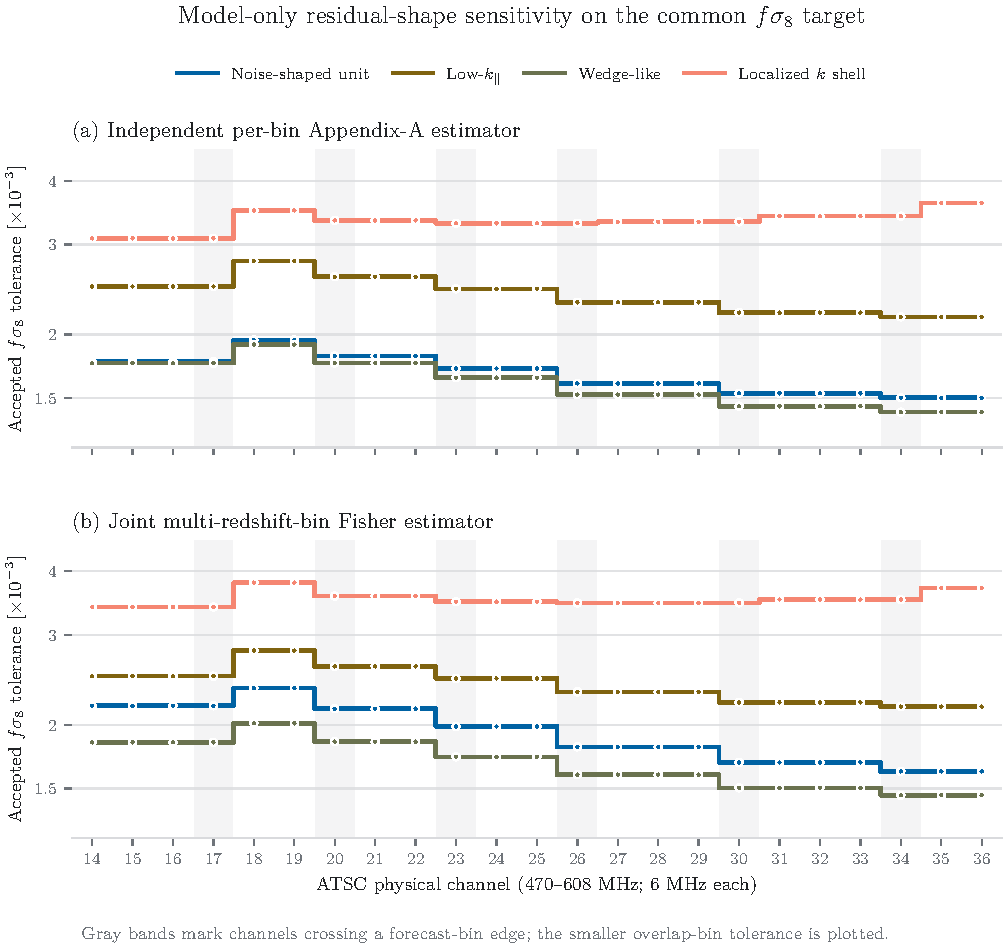
\includegraphics[width=0.98\linewidth]{figs/fig_bao_template_tolerances.pdf}
\caption[Analytic residual-shape tolerance across ATSC channels]{Model-only
residual-amplitude tolerance on the common $f\sigma_8$ target at one on-sky
year, mapped to ATSC channels 14--36.  Panel (a) uses the independent per-bin
estimator and panel (b) the joint multi-redshift-bin Fisher estimator.  For a
channel crossing a redshift-bin edge, the plotted value is the smaller accepted
tolerance over every bin with non-zero frequency overlap.  All plotted
$f\sigma_8$ points pass the $\pm10\%$ stability gate.  The four curves are
analytic unit-response hypotheses normalized to contemporaneous thermal-noise
power, not empirically inferred template probabilities or measured channel
residuals.  Frequency-, baseline-, and sidereal-dependent visibility templates
remain explicitly data-dependent and incomplete.}
\label{fig:tolerance:template-tolerances}
\end{figure}

The executed estimator/time triplet is
\emph{per-bin noise-normalized}, \emph{combined noise-normalized}, and
\emph{combined fixed-physical}; no independent per-bin fixed-physical ledger is
claimed.  The two combined residual-time conventions were run at $0.9$, $1.0$,
and $1.1$ times the one-year reference. For every accepted and refused point, the fixed-physical
and contemporaneous-noise families use the same bank-native response and agree
exactly at the reference time; away from it, the fixed-physical response gains
the declared $t/t_{\rm ref}$ multiplier while its tolerance loses the same
factor.  This verifies the implementation of the two definitions without
pretending that they describe the same physical residual away from the
reference time.

The status consequence is deliberately restrained.  None of the existing
channel-policy labels or within-channel mask rankings is changed merely by
choosing the loosest analytic curve: the archive supplies no empirical
probability that the residual is a localized shell rather than wedge-like, and
the scalar proxy does not expose the baseline, frequency, or sidereal
coordinates needed to decide.  The completion release therefore marks the
frequency-localized, baseline-localized, and sidereal-coherent empirical rows
as data-dependent refusals.  Those are the remaining template gates; the
combined estimator and the four code-supported analytic families are complete.


For continuity with the channel screen, applying the binding per-bin, noise-shaped value $r_{\text{tol}}=1.5\times10^{-3}$ to the policies of Section~\ref{sec:tolerance:policy}, through the scalar chain and unity-transfer closure, produces the stringent conditional result below.  It is the common reference case, not a claim that the completed analytic envelope has selected the real residual's shape. Figure~\ref{fig:tolerance:case} shows the policy ordering at the target time on one channel, while Fig.~\ref{fig:tolerance:convergence} shows the behavior of the particular noise-normalized time family used by that screen.  Neither figure is a substitute for the visibility-transfer and empirical-template tests stated above.

\emph{Within the scalar screening model, no evaluated policy clears the binding growth-rate tolerance on a channel with a defensible kept-frame floor, the pilot proxy evaluated as a stand-in at the survey flag.} On the best-constrained channel of the superseded products --- channel 33, whose floor and correlation-time bound were both data-derived --- keeping everything gave \rerun{$r_{\rm proxy}=2.35$}, the MAD cut \rerun{$2.38$}, spectral kurtosis \rerun{$0.573$}, and the pilot proxy \rerun{$0.0359$}: against $1.5\times10^{-3}$ these are \rerun{$1{,}566\times$, $1{,}587\times$, $382\times$, and $24\times$} over.  These are not caveat-free visibility verdicts: they inherit the proxy transfer, unity coefficients, noise-shaped template, and per-bin estimator.  What survives that verdict is the ordering: the pilot proxy leaves a residual \rerun{16 to 66} times smaller than the best alternative on the same frames, and \rerun{44 to 65} times smaller than keeping the data; within this common scalar screen, no other evaluated policy is within one and a half orders of magnitude of it.  The per-channel result of the same calculation at the tolerance-selected fine operating point is Table~\ref{tab:tolerance:channels}.
\stub{v5 archive rerun}{Replace the channel-33 example numbers with the current-era values from Table~\ref{tab:tolerance:channels}, and state the across-channel range of the pilot-proxy-over-best-alternative ratio.}

\begin{figure}[t]
\centering
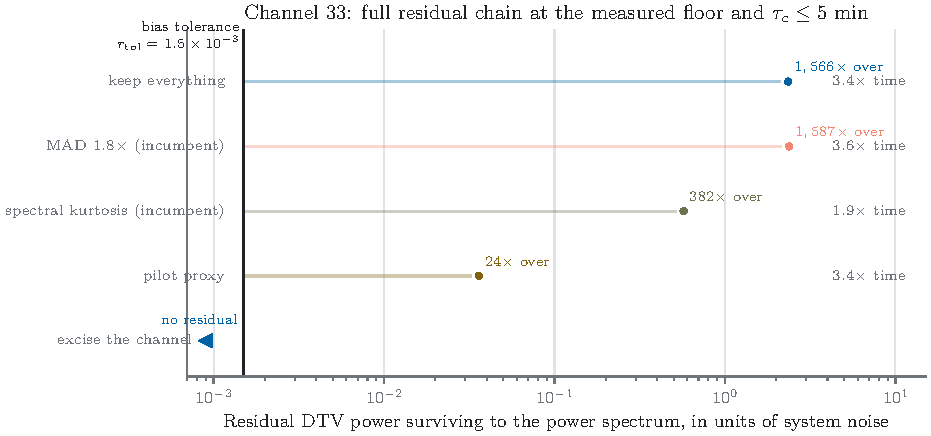
\includegraphics[width=0.98\linewidth]{figs/fig_bao_the_case.pdf}
\caption[Every policy on the residual axis, one channel]{Every policy on the axis that decides between them, for one channel whose kept-frame floor and correlation-time bound are both constrained by data (channel 33 on the superseded products). The rule is the bias tolerance of Eq.~\eqref{eq:tolerance:rtol} at the adopted $\zeta=1$ convention. Integration time rides as an annotation rather than a second axis, because every failing policy fails on residual whatever its time cost. Excision sits at the left edge with no residual and no measurement: it wins the axis shown and loses the one that cannot be drawn. The pilot proxy is the best of the four by a factor of \rerun{sixteen} and still lands \rerun{$24\times$} outside.
\stub{v5 archive rerun}{Regenerate for the same channel on its current era at the selected $(\rho^\star,\eta^\star)$, with the survey-flag stand-in shown only as a reference.}}
\label{fig:tolerance:case}
\end{figure}

\begin{figure}[t]
\centering
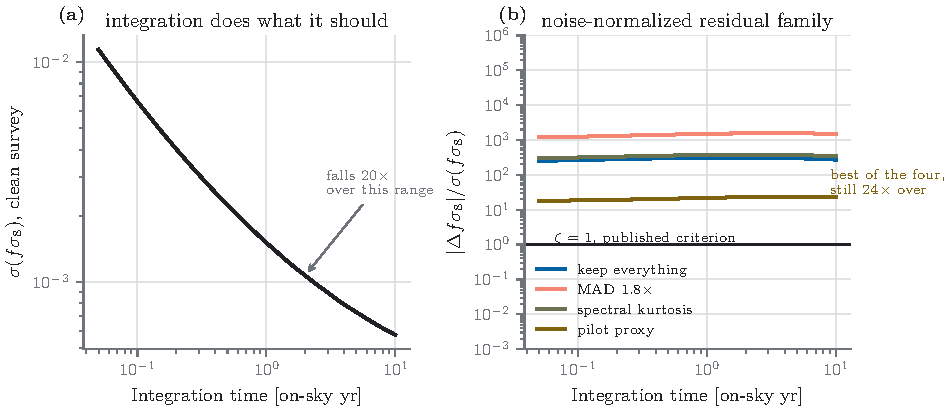
\includegraphics[width=0.98\linewidth]{figs/fig_bao_convergence.pdf}
\caption[Time scaling under the current residual normalization]{Time scaling under the current noise-normalized residual family.  At each plotted integration time the template amplitude is defined relative to that time's thermal-noise covariance, so the induced bias and $\sigma(f\sigma_8)$ fall at similar rates and their ratio is nearly flat.  This figure does not describe a fixed physical contaminant, whose significance can grow as the statistical error shrinks.  The tolerance used for the channel decisions is therefore defined at the fixed target time $T^\ast$ rather than inferred from this curve as a universal convergence law.  The artwork's ``published criterion'' label is shorthand for the adopted $\zeta=1$ convention; it is not a claim of universal status.}
\label{fig:tolerance:convergence}
\end{figure}

\subsection*{Spending the tolerance}

The loop is only closed if the tolerance can be converted into an operating point, so the last step is to spend it, and the coarse sweep on one well-measured channel shows the shape of the problem before Section~\ref{sec:tolerance:thresholds} does it properly on the fine axis for every channel. Sweeping the coarse multiplier $\eta_c$ on channel 33 and carrying each setting through Eq.~\eqref{eq:tolerance:chain} gave, on the superseded products:

\begin{center}
\begin{tabular}{lccccc}
\toprule
$\eta_c$ & $1$ (floor) & $1.2$ & $1.5$ & $2$ & $5$ \\
\midrule
masked fraction $f$ & \rerun{$0.805$} & \rerun{$0.158$} & \rerun{$0.092$} & \rerun{$0.048$} & \rerun{$0.007$} \\
kept-frame shelf (dB) & \rerun{$-45.3$} & \rerun{$-34.8$} & \rerun{$-33.3$} & \rerun{$-31.6$} & \rerun{$-29.6$} \\
residual $r_{\rm proxy}$ & \rerun{$0.0334$} & \rerun{$0.369$} & \rerun{$0.524$} & \rerun{$0.772$} & \rerun{$1.24$} \\
$r_{\rm proxy}/r_{\text{tol}}$ & \rerun{$22$} & \rerun{$246$} & \rerun{$349$} & \rerun{$514$} & \rerun{$828$} \\
\bottomrule
\end{tabular}
\end{center}

The detection-floor setting is the best available coarse setting by a wide margin, and nothing above it competes: relaxing $\eta_c$ by a fifth recovers \rerun{$65\%$} of the data and multiplies the residual by \rerun{eleven}. For this channel and this scalar-chain sweep there is no competitive intermediate coarse operating point: either the detectable-pilot population is removed and the retained set sits near the measured floor, or the readmitted frames dominate the mean.  This sharpens --- and partly corrects --- the operating-point argument of Section~\ref{sec:pipeline:decision}. The $21.6$~dB proxy margin of Eq.~\eqref{eq:proxymargin} is real and still computable in advance from the broadcast standard. What that section could not know is that the margin is not free to spend, because the residual chain consumes it: on this channel the chain multiplies the kept-frame floor by \rerun{$+30.5$~dB} \emph{net} --- the coherence amplification already discounted by the ground filter, with no delay credit claimed --- against a $21.6$~dB margin. The general claim survives --- a threshold should be set by the contamination-residual tolerance rather than by $P_{\text{fa}}$ --- but on a channel whose residual outlives the common-mode filter the tolerance-set threshold and the detection floor coincide.  Whether the fine axis, which decides about $10$~dB deeper, opens a competitive intermediate point is exactly what the per-channel selection of Section~\ref{sec:tolerance:thresholds} measures rather than assumes.

\subsection*{What $\zeta$ means, and why the verdict does not depend on it}

The form of Eq.~\eqref{eq:tolerance:rtol} is standard. Requiring that a systematic shift stay below the statistical error it competes with is the standard criterion for propagating an unmodelled effect through a Fisher forecast; Amara \& R\'efr\'egier state it as
\begin{equation}
\label{eq:tolerance:arcrit}
b[\hat{p}_i] \;\le\; \sigma[\hat{p}_i]
\end{equation}
for the parameters of interest, and use the ratio $b/\sigma$ as the metric throughout \cite{amara2008}. Equation~\eqref{eq:tolerance:rtol} is that criterion with an explicit slack factor, and \emph{this work adopts $\zeta = 1$} as a conventional, deliberately permissive systematic-budget criterion inspired by that literature.  It is neither a universal community threshold nor a frequentist coverage guarantee.  A collaboration must set $\zeta$ from its complete error budget; the question answered here is whether the measurement clears the stated choice.

It is still worth saying what $\zeta$ means, because a survey may want to set its own. If $\Delta$ is treated as a deterministic bias and $\sigma$ as the standard deviation of the statistical error, their quadratic combination $\sqrt{\sigma^2+\Delta^2}=\sigma\sqrt{1+\zeta^2}$ is the root-mean-square error (RMSE), not a larger statistical uncertainty.  Relative to $\sigma$, that RMSE is larger by $41\%$ at the adopted $\zeta = 1$, $11.8\%$ at $0.5$, $4.4\%$ at $0.3$, and $0.5\%$ at $0.1$. A second reading bounds it from the other side, since DTV is one line in a budget: a survey holding its total systematic below $0.5\sigma$ across $N$ independent terms of comparable size allots each $0.5/\sqrt{N}$ --- $0.289$ at $N = 3$, $0.158$ at $N = 10$. A collaboration with a long systematics list should therefore run tighter than the permissive convention used for this screen, and the framework computes $r_{\text{tol}}(\zeta)$ for whatever value is set; it does not presume to set it. Tightening to $\zeta = 0.3$, three times stricter, moves the binding tolerance from $1.5 \times 10^{-3}$ to $4.5 \times 10^{-4}$.

The policy ordering is not load-bearing on this choice. $r_{\text{tol}}$ scales linearly in $\zeta$, while on the example channel the pilot proxy leaves \rerun{$0.0359$} and the best alternative leaves \rerun{$0.573$}, a factor of \rerun{$16$} apart, so no value of $\zeta$ reorders them.  Absolute pass/fail is mathematically different: the proxy would pass only at \rerun{$\zeta \ge 24$} and the best alternative only at \rerun{$\zeta \ge 382$}.  Thus the failing verdict is unchanged throughout any defensible systematic budget of order unity or smaller, but it is not claimed to be invariant under arbitrarily large $\zeta$.

\textit{A note on two dimensionless factors that are easy to confuse.} This section's $\zeta$ and the detector's $\mu_0$ are unrelated, and only $\mu_0$ is derived.  The manifest value $\mu_0=2\lVert\mathbf w_0\rVert^2/(\lVert\mathbf w_1\rVert^2+\lVert\mathbf w_2\rVert^2)$ is an exact rational consequence of the quantized weight-bank norms (Section~\ref{sec:param:refs}); under the declared white, isotropic null it is the ratio of expected target and reference powers.  Arithmetic exactness does not make it the exact finite-sample mean of $F$, nor does it establish the empirical null distribution.  $\zeta$, by contrast, is a requirement a collaboration sets in the Fisher forecast and answers a science question --- \emph{how much bias can the measurement absorb?} The two meet only through the loop this chapter constructs: $\zeta$ fixes $r_{\text{tol}}$, preparation produces the calibrated residual-score histograms, and the selector returns the per-channel $(\rho,\eta)$ used by the implemented decision. Thus $\mu_0$ is a derived scale factor, while $\eta$ and $\zeta$ encode calibrated operating and science-budget choices.

\section{The Forecast-Selected Operating Point}
\label{sec:tolerance:thresholds}

Section~\ref{sec:pipeline:decision} set no threshold during the survey and promised that the operating point would be tolerance-derived once the forecast matured. RFIsher's threshold stage is that replacement, and its interface separates preparation from selection. Preparation operates only on the current era of Section~\ref{sec:calibration:eras}; earlier eras remain provenance rather than threshold candidates. It requires already-filtered valid rows, establishes the anchor and bulk, applies floor and correlation conventions, calibrates the proxy-to-residual transfers, and compares the complete candidate surface across calendar halves.  A versioned decision record travels with the result: every consequential value is classified as derived, locked, provisional, open, conditional, or historical, with its rationale and sensitivity values.  The evidence-bearing selector refuses a stale decision digest, a non-latest era, unequal exposure, non-additive calibration, an unconfigured or failed early/late drift screen, or inadequate transfer evidence. Its numerical payload is the complete mapping
\[
\mathcal H=\{\rho:\mathcal H_\rho\},\qquad
\mathcal H_\rho=\left(
|\mathcal B|,
\{\eta_{\rho k}\}_{k=1}^{J_\rho},
\{(n_{\rho j},R^{\rm sys}_{\rho j},[R^{\rm var}_{\rho j}])\}_{j=0}^{J_\rho}
\right),
\]
where $|\mathcal B|$ validates the one-based rank and gives $q_\rho=\rho/(|\mathcal B|+1)$, the ordered $\eta_{\rho k}$ are candidate score boundaries, the $n$ fields are frame counts, and the two $R$ fields are additive calibrated residual totals. The detector's stored \texttt{cfar\_rank} is a zero-based array index, so $\rho=\texttt{cfar\_rank}+1$. Bins zero through $J_\rho-1$ end at the candidate boundaries; bin $J_\rho$ is the required overflow above the last candidate. The variance total is optional; the coherent total is required. Completeness means that every accepted equal-duration, equal-exposure frame in the prepared era contributes to exactly one bin for every candidate $\rho$. Across ranks, the accepted population, usable bulk size, full coherent total, and optional variance basis and full total must agree.  A deployable fine-stage family contains every one-based rank from $1$ through the minimum usable-bulk count supported by all accepted frames. For each rank, the authoritative threshold grid begins at the Q16 integer $\eta_{q16}=1$ --- the real multiplier $2^{-16}$, not unity --- and includes every unique observed Q16 multiplier at which a frame's exact integer decision changes, provided it fits the deployed unsigned 64-bit field. A frame whose required multiplier overflows the deployable field carries the $2^{64}$ sentinel --- it is masked by every deployable threshold, hence ``always masked'' --- and that value is a frame label, not a candidate threshold; it is excluded from the grid. (The threshold endpoints themselves run the other way: $\eta \to \infty$ keeps every frame and $\eta = 0$ masks every frame with a positive statistic.) Floating $\eta=\eta_{q16}/2^{16}$ is therefore only a display value for an exact empirical staircase, not an interpolated or geometrically spaced grid.

The selector receives only $\mathcal H$ and the science tolerance. For a candidate $(\rho,\eta)$ it derives
\begin{align}
N_\rho &= \sum_{j=0}^{J_\rho} n_{\rho j}, &
K(\rho,\eta_{\rho k}) &= \sum_{j=0}^{k-1}n_{\rho j},\\
f(\rho,\eta_{\rho k}) &= 1-\frac{K(\rho,\eta_{\rho k})}{N_\rho}, &
r_{\rm sys}(\rho,\eta_{\rho k}) &=
\frac{\sum_{j=0}^{k-1}R^{\rm sys}_{\rho j}}
{K(\rho,\eta_{\rho k})},
\end{align}
and derives $r_{\rm var}$ by the same cumulative sum when variance totals are present. Thus the sample count and masked fraction are properties of the histogram, not additional inputs. A candidate must retain at least thirty frames. Each feasible point has cost
\[
\mathcal C(\rho,\eta)=\frac{1 + r_{\rm var}(\rho,\eta)}{1 - f(\rho,\eta)},
\qquad r_{\rm sys}(\rho,\eta) \le r_{\rm tol}.
\]
The selector treats $r_{\rm tol}$ as a generic caller-supplied science tolerance. The per-channel selection below supplies the stable dilation tolerance of the channel's own redshift bin at $\zeta=1$ --- the operable tier, since it is the requirement a no-delay-filter analysis can meet --- and reports the growth-rate margin alongside; that is one use of the interface, not part of its general contract. If variance totals are unavailable, $r_{\rm var}$ remains unavailable and the declared cost reduces to the masking term; the selector does not invent a transfer. Let $\mathcal C_{\min}$ be the smallest feasible cost. Within the declared provisional plateau $\mathcal C\le1.02\mathcal C_{\min}$, the selected pair is the candidate with lexicographically smallest $(r_{\rm sys},f,\rho,\eta)$. The thirty-frame support floor and the two-percent plateau are project policies, not statistical constants; registered sensitivity values are $(30,50,100)$ frames and plateau factors $(1.00,1.01,1.02,1.05)$. Era dates, rejected-frame ledgers, and calibration diagnostics remain attached provenance, not arguments to this calculation. The adopted $\zeta=1$ run and the smaller values $(0.5,0.3,0.1)$ reuse the same histograms; changing $\zeta$ changes only the supplied tolerance.

The implemented within-era check is a deterministic early/late point-estimate drift screen, not an equivalence test. It fixes one calibration, splits the latest era at its calendar midpoint, and compares the cost and systematic-residual response at every selector-evaluable pair; pooled candidates below the thirty-frame support floor are excluded first. Each half must contain at least six observed months and span at least 270 elapsed days between its first and last accepted timestamps; the span is not inferred from month labels. Those are provisional archive guardrails. The precision-based retained-frame floor for each half and the maximum acceptable early/late cost and systematic-residual ratios are deliberately unset: the former must follow estimator precision, the cost margin must follow science materiality, and the systematic margin must follow transfer uncertainty or a residual-budget allocation. Registered sensitivity probes of $(15,30,50,100)$ retained frames, cost ratios $(1.02,1.05,1.10)$, and systematic-residual ratios $(1.05,1.10,1.20)$ are not adopted limits. A half-population support failure returns an insufficient-support refusal before unset margins can return an unconfigured refusal. Even after the margins are chosen, point-estimate ratios alone cannot support an operational stability claim: acquisition- or day-blocked uncertainty must be shown to lie within the justified margins \cite{kunsch1989,schuirmann1987}. Under the current unity shelf-to-science transfer, a caller may request a labelled screening result, but cannot promote it to an operational calibration.

The result of that selection for every channel is Table~\ref{tab:tolerance:eta}: one fine operating point per channel, selected on its current era's null distribution, with the rank as an optional second degree of freedom. Because the survey products retain the exact integer fine powers, the selected pair is applied to every frame of the era exactly, and the masked fraction, kept-frame floor, and residual in the table are measurements at that operating point rather than projections from the coarse rule.

\stubtab{v5 archive rerun}{One row per channel 14--36: current era; $|\mathcal B|$; selected rank $\rho^\star$ (and normalized rank $q_\rho$) and multiplier $\eta^\star$ (display value and exact $\eta^\star_{q16}$); masked fraction $f$ at that point; kept-frame floor (dB) and its population; $r_{\rm proxy}$; the operable-tier tolerance $r_{\rm tol}$ of the channel's bin and the ratio $R = r_{\rm sys}/r_{\rm tol}$ ($R \le 1$ passes); cost $\mathcal C$ of Eq.~\eqref{eq:tolerance:teff}; plateau width; and the selector's status (feasible, occupancy-wall, no feasible point, refused with reason).  Channels whose $\tau_c$ is refused carry bounds, marked as such.}{Tolerance-selected fine operating points $(\rho^\star,\eta^\star)$ for every channel, from RFIsher on the current-era null distribution.\label{tab:tolerance:eta}}

Per-channel selection against the bin tolerance is conservative \emph{within} a bin, because $r$ is an intensive quantity that combines across the channels of a bin with bandwidth weights rather than adding, so channels each at or below tolerance leave the bin at or below tolerance; it is not automatically conservative \emph{across} bins in the joint estimator. The closing evaluation therefore propagates the full 23-channel residual vector through the combined-bin estimator once, at the selected operating points, as the survey-wide bias check (a row of Table~\ref{tab:tolerance:channels}); a failure there is allocated back to channels as a tightened per-channel tolerance, not hidden. Two limiting regimes appear whenever the whole band is drawn in one plane. Figure~\ref{fig:tolerance:twowalls} plots every channel as a curve and every threshold as a point in the $(f,\ r_{\rm proxy}/r_{\rm tol})$ plane. The \emph{bias wall} is where this detector and calibration cannot demonstrate a sufficiently clean retained population; the \emph{occupancy wall} is where the transmitter is present in nearly every archived frame. A channel is a screening-model recovery candidate only when its curve enters the box between them, and the two walls are nearly mutually exclusive in any one era because both are driven by the same variable --- duty cycle --- pulled in opposite directions. A formally feasible point at the occupancy wall (a masked fraction near unity at a time cost of hundreds) is vacuous, and it is the cost axis that unmasks it; that is why the selector optimizes cost under a residual constraint rather than residual alone. Floating $\eta$ is display-only and is never converted back to Q16; runtime-bundle packaging exports the selected exact $\eta^\star_{q16}$ unchanged.

\begin{figure}[t]
\centering
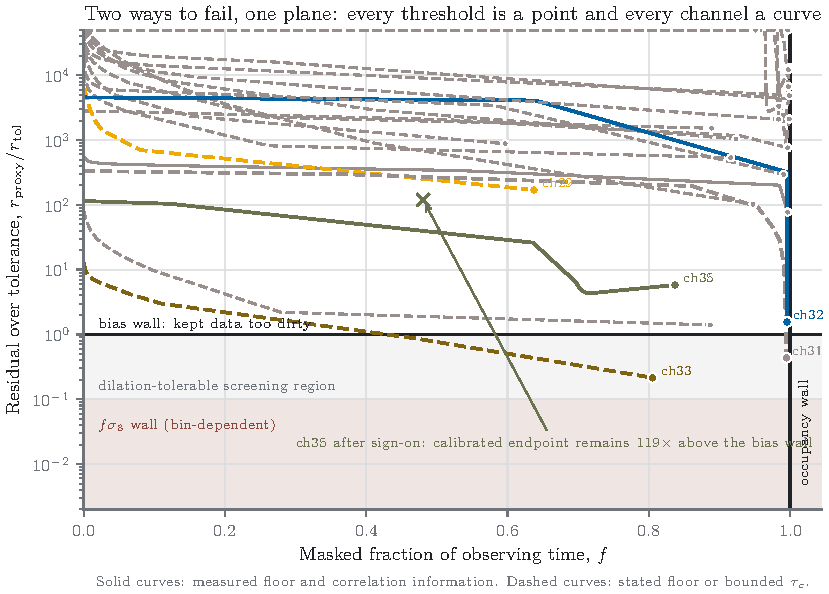
\includegraphics[width=0.98\linewidth]{figs/fig_bao_two_walls.pdf}
\caption[The two walls: every channel in the (masked fraction, residual) plane]{Every channel is a curve and every threshold is a point in the $(f,\ r_{\rm proxy}/r_{\rm tol})$ plane, with the tolerance on the stable dilation tier of the channel's own redshift bin. The two tolerance boundaries are the two failure modes of this chapter: the \emph{bias wall} (top edge: kept data too dirty) and the \emph{occupancy wall} (right edge: nothing left to keep). Raising $\eta$ walks a curve right-to-left. Dashed curves carry a stated (rather than measured) floor or a $\tau_c$ bound --- a refused $\tau_c$ takes no ground-filter credit, so those curves are upper bounds; the shaded band is where the $f\sigma_8$ wall falls, 10--25$\times$ lower depending on bin.
\stub{v5 archive rerun}{Regenerate on the fine axis from the current-era histogram families: one curve per channel at its selected $\rho^\star$, the selected $\eta^\star$ marked on each, and the survey-flag stand-in for reference. The figure shown is the coarse-rule version from the superseded products.}}
\label{fig:tolerance:twowalls}
\end{figure}

\section{The Delay Filter Booked on Both Sides}
\label{sec:tolerance:worlds}

Every verdict so far declines the delay filter's help, because the forecast convention carries no filter (Section~\ref{sec:tolerance:chain}). That is the conservative bookkeeping, but it leaves the growth rate unpriced under the analysis configuration that would actually measure BAO, and the framework can do better than a one-sided bound: the filter can be booked \emph{self-consistently}, on both sides of the calculation at once. A delay cut $\tau_{\rm cut}$ maps to a parallel-wavenumber cut through Eq.~\eqref{eq:tolerance:kpar} --- in the forecast's own foreground switch, a mode exclusion at $k_{\rm FG} = \tau_{\rm cut} \times 400$~MHz in grid units --- so each candidate cut defines a \emph{world}: the Fisher bank loses the modes below the cut (tolerances re-derived, the Fisher response-stability gate of Eq.~\eqref{eq:tolerance:stability} re-applied), and the residual chain gains the matching shelf suppression from the same $\tau \leftrightarrow k_\parallel$ mapping. Nothing is invented: the cut values are the published $200$~ns and the two BAO-preserving design points any analysis in this band faces ($55$~ns preserving the first acoustic peak, $110$~ns the second), and the suppressions are the same $3.6$/$8.2$/$11.4$~dB the chain already carries as unbanked bounds. One guardrail keeps the exercise honest: the worlds model the \emph{mode-cut geometry} only --- what sensitivity the analysis gives up and what shelf power the cut removes --- never the filter's foreground-removal performance, which remains another subsystem's contribution.

\begin{table}[t]
\centering
\caption[Three delay-filter screening worlds]{Three screening worlds (example rows from the superseded products; to be regenerated for every channel at its selected operating point): the growth-rate ratio $R = r_{\rm sys}/r_{\rm tol}(f\sigma_8)$ ($R \le 1$ passes; the one direction used throughout), with the residual at the selected operating point, the measured floor and refusal conventions, and each world's tolerances re-derived from its own mode-cut bank with the Fisher response-stability gate of Eq.~\eqref{eq:tolerance:stability} re-applied. Channel 33 is the only evaluated row that clears both dilations in every world. Ratios $\le 1$ (bold) pass. Channels 35 and 29 are shown for contrast; neither clears all three parameters in any world. Channel 35's parallel dilation alone passes at $110$~ns, while its perpendicular dilation and growth rate still fail. Channel 32 has no quoted margin because its transmitter-on era retains only 16 frames at $\eta=1$, below the 30-frame population gate. All values are direct outputs of the four matched bias-response banks.}
\label{tab:tolerance:worlds}
\begin{tabular}{lcccc}
\toprule
$f\sigma_8$ margin & no filter & $55$~ns ($3.6$~dB) & $110$~ns ($8.2$~dB) & $200$~ns ($11.4$~dB) \\
\midrule
ch\,33 & \rerun{$2.2$} & \rerun{$\mathbf{0.83}$} & \rerun{$\mathbf{0.24}$} & \rerun{$\mathbf{0.067}$} \\
ch\,35 & \rerun{$135$} & \rerun{$53$} & \rerun{$14$} & \rerun{$3.2$} \\
ch\,32 & \multicolumn{4}{c}{not evaluated: $16<30$ kept frames at $\eta=1$ in its transmitter-on era} \\
ch\,29 & fails all & fails all & fails all & fails all ($\alpha_\perp$ $3.2\times$ over) \\
\bottomrule
\end{tabular}
\stub{v5 archive rerun}{Regenerate for all 23 channels at their selected $(\rho^\star,\eta^\star)$, one row per channel, four worlds per row, with the dilation margins in a companion table.}
\end{table}

Table~\ref{tab:tolerance:worlds} is where the screening model's positive results live, and it shows what booking the filter self-consistently does. At the $110$~ns design cut, on the superseded products, the unity-transfer, noise-shaped calculation placed all three parameters inside tolerance on the one channel whose floor and coherence were both measured, with a growth-rate ratio of \rerun{$R = 0.24$}, while channels on the occupancy wall gained nothing from any cut. Two structural features of the table deserve note. The $f\sigma_8$ tolerance itself loosens with cut depth --- from $1.5\times10^{-3}$ with no filter to $3.7\times10^{-3}$ at the deployed cut --- because the cut removes exactly the smooth low-$k_\parallel$ modes through which an additive residual counterfeits amplitude: the filter protects the growth rate twice, once by suppressing the residual and once by excising the modes it damages most. And the deployed $200$~ns column, though it posts the largest margins, is not an operating point for this science --- it is the configuration the hybrid demonstration states excludes BAO sensitivity \cite{chime2024hybrid} --- which is why the $110$~ns world is the operative one, and why the note of Section~\ref{sec:tolerance:chain} matters: the cleanliness experience earned at $200$~ns overstates what the $110$~ns world will exhibit by the $3.2$~dB difference, roughly a factor of two in residual. Filtering solves only the filtering-shaped problem: a channel whose failure is a $\tau_c$ refusal belongs to the contiguous campaign, not to any choice of cut. This is evidence that a joint mask--filter configuration is worth validating on the channels that survive; it is not yet a visibility-domain recovery claim, and it remains conditional on the across-allocation proxy, $g_{\rm var}$ and $g_{\rm sys}$, empirical residual-shape selection, a cut-specific evaluation with the combined-bin estimator, and era-specific holdout tests.

\section{An Archive Is Not One Era}
\label{sec:tolerance:eras}

Every fraction quoted so far is evaluated on the channel's current era, and Section~\ref{sec:calibration:eras} is where that era is identified; this section records why the discipline is load-bearing for the verdicts rather than a refinement of them. The broadcast environment changed measurably inside the archive span: the FCC incentive-auction repack was still relocating stations through mid-2020, individual transmitters signed on and off, and one channel's collection was curtailed by the observatory on account of the contamination itself. On the superseded products the archive-average masked fraction described no physical state on most of the band --- a station departure moved one channel from \rerun{$99.8\%$} masked to \rerun{$59\%$}, a switch-on moved another from \rerun{$46\%$} to \rerun{$94\%$}, and the anchors moved with the stations, by \rerun{11} and \rerun{29} fine bins respectively, because they were different transmitters at different offsets rather than drift.

The era-mixture trap is worth stating in the residual chain's own terms because it is the clearest argument for the per-era rows of Table~\ref{tab:tolerance:channels}. Evaluated era-blind, a channel with a dated sign-off can \emph{formally pass} the dilation tier, because the sign-off step itself is classified into the DC and inter-day shares that the ground filter removes --- the transmitter's death masquerades as filterable structure --- and an era-straddling structure function can even return a spuriously ``measured'' $\tau_c$ across the step. Those numbers are artefacts of averaging across a transition, not verdicts. A current policy is therefore prepared from the latest accepted station-state era; the absolute start and end dates, transition evidence, and rejected earlier eras remain in provenance, and the selector receives the resulting histogram mapping, not those dates or the older distributions. A new transition anywhere in the band requires a new latest-era mapping and resets the empirical operating-point evidence, not the weight-norm arithmetic --- one more reason the monitoring taps of Chapter~\ref{sec:deployment} stay on.

\section{Channel Verdicts, and What the Archive Cannot Settle}
\label{sec:tolerance:verdicts}

Table~\ref{tab:tolerance:channels} carries every channel through the residual chain of Section~\ref{sec:tolerance:chain} term by term, on its current era, at the tolerance-selected operating point of Table~\ref{tab:tolerance:eta}, on one stated basis: unity pilot-to-shelf transfer, no delay credit, the noise-shaped template, the per-bin estimator, and $r_{\rm tol} = 1.5\times10^{-3}$ for the growth rate at $\zeta = 1$. The reported levels are pilot-derived per-coarse-channel screening values transferred across the $15.36$-bin allocation by the model of Section~\ref{sec:tolerance:footprint}; they are not direct measurements in every protected bin. ``cap'' marks channels where the correlation-time estimator refused and the chain is evaluated at the sidereal-day bound, so their residuals are upper bounds rather than measurements; on cap channels the chain takes no ground-filter credit, because the non-stationarity that defeats the timescale estimator defeats the variance split too, so all surviving shelf power is booked at the cap and the intra-day share and ground-filter rows are reported as measured description rather than applied credit. A channel whose current era is a transmitter-off era is evaluated on that era, with its floor taken as the 90th percentile of the off-era shelf.

\stubtab{v5 archive rerun}{One row per channel 14--36 with the short columns below; the term-by-term evidence ledger behind each row goes to Appendix~\ref{app:archive-diagnostics} beside the channel's plate rather than into a 23-column table. Columns: allocation (MHz); redshift span; monitored bin (MHz); current era; flag rate (occupancy indicator) and masked fraction at $(\rho^\star,\eta^\star)$; on-air shelf (dB); null frames; kept-frame floor (dB); intra-day share; ground filter (dB); $\tau_c$ outcome; $r_{\rm keep}$; $r_{\rm proxy}$ at the selected point; $r_{\rm proxy}/r_{\rm tol}$ on the dilation tier and on $f\sigma_8$; and the screening class (recovery candidate, measurement-bound, occupancy-wall excision candidate, or off-era).}{The scalar residual chain, term by term, for every channel on its current era at its selected operating point.\label{tab:tolerance:channels}}

The channels do not distribute evenly across the framework's possible outcomes, and the pattern is more informative than any single channel. Three screening outcomes are possible per channel: the residual lies inside tolerance under all required validation gates; the crossover exists but depends on an unresolved measurement; or no admissible operating point is found and the channel becomes an excision candidate. On the superseded products the three classes were all populated, and the reasons a channel landed in each were the physics rather than the detector: occupancy-pinned channels with no null population at all sat on the occupancy wall; the trace family --- faint shelves with intra-day-heavy shares through weak ground filters --- had verdicts hostage to refused correlation times and thermal-end residuals that passed trivially, so that the bracket, not the shelf, was their entire verdict; the dated sign-off channels supplied the most defensible floors of all from their off eras; and the one channel with both a measured floor and a bounded $\tau_c$ was the one on which the calculation was a measurement end to end.
\stub{v5 archive rerun}{Two or three paragraphs walking the table: which channels admit a recovery candidate on the dilation tier at their selected point, which are measurement-bound and on what (floor or $\tau_c$), which are occupancy-wall excision candidates, and which are evaluated on an off era; name the best-constrained channel and the channel whose verdict hangs most completely on a pending measurement.}

\subsection*{What would close the gap}

A negative verdict earns its keep by saying which measurement to go and get, so it is worth walking the remaining distance in terms that can be checked. Three levers are available and they bind differently per channel. The first is the \emph{decision axis}: the fine designated-set decision, applied exactly from the retained integer powers, is what Table~\ref{tab:tolerance:channels} reports, and where a channel's excess is \emph{spread} across the fine axis rather than concentrated at one anchor (channel 33's structure on the superseded products, where a narrow window at any single anchor covered only \rerun{$2$--$5\%$} of its coarse-masked frames), no single-line sensitivity result transfers until that wide structure is diagnosed by the flanking-bin census. The second lever is the \emph{delay filter}, whose credit this chapter declines to claim on scope grounds but which the eventual analysis will apply, and which Section~\ref{sec:tolerance:worlds} books self-consistently rather than as a one-sided conditional. The third is $\tau_c$ itself: on a cap channel a measured correlation time restores both the timescale and the ground-filter credit the refusal withholds, and a minutes-scale measurement moves such a channel's bound by three to four orders of magnitude; the contiguous-scan campaign is specified for the large-null, coherence-limited channels first for exactly this reason. These bounds and projections identify what can close each gap; they do not pre-approve a channel recovery verdict. A channel that would need a floor below what any combination of the three levers reaches --- channel 36 on the superseded products needed \rerun{$-91$~dB} --- is an excision candidate, and the framework's contribution there is a measured basis for saying so rather than an assumption that every archive-average channel can be integrated through.

\subsection*{What the archive cannot settle}

Four limits of the triggered archive are structural, and stating them fixes the requirements of the closing campaign. First, \emph{cadence}: its snapshots cap block statistics at the longest capture (\rerun{$1.38$~s}), so the incumbent comparison at its native few-second cadence, and any $\tau_c$ between seconds and the acquisition spacing, are unmeasurable here. Second, \emph{null populations}: a channel that is always on in its current era has no per-frame null population, and without a transmitter-off era its masked residual cannot be measured at all --- the fine stage's per-frame null re-decision is the unlock where the coarse rule left none. Third, \emph{refusals are load-bearing}: on the channels whose correlation times are refused the refusal is worth three to five orders of magnitude in the verdict, and a framework that extrapolated $\tau_c$ would have produced confident answers the data cannot support. Fourth, \emph{footprint}: the products record only the monitored bin, so the proxy's transfer across the allocation is assumed rather than verified (Section~\ref{sec:tolerance:footprint}). None of the positive screening classes becomes a final recovery verdict until the across-allocation and visibility transfers are measured, an empirical residual template is selected and propagated through the combined estimator, and the blocked-holdout gate passes. What is complete here is the auditable machinery: the tolerance is computable, policy costs and residual screens are reported separately, refusal states remain visible, and every remaining measurement is tied to a channel, era, and decision it can change.

\subsection*{The per-channel disposition}

The survey handover deliverable to the collaboration is a screening-level disposition for each of the 354 CHIME coarse channels in the declared inclusive edge-bin range \texttt{freq\_id}=492--845 associated with the ATSC~1.0 allocation ($470$--$608$~MHz). This is a \emph{policy recommendation at screening level}, layered on the evidence of this chapter without altering it, under two rules adopted for the handover: allocations without a live carrier keep all of their channels at the channel's selected operating point; excised allocations discard their interiors but keep any boundary channel shared with a kept allocation and keep their pilot-bin channel as a monitoring tap. One further rule follows from the inclusive posture: an edge shared by \emph{two} excised allocations is discarded. The handover's \emph{policy status} and the residual chain's \emph{science status} are intentionally separate columns of judgment: a channel whose collection was curtailed remains a science-side excision candidate on its latest observed, near-fully-occupied archive, and the policy discards its interior conservatively, without either statement asserting that a live carrier has been measured there since. The inclusive posture generally is an asymmetry argument: the mask is software and the archive stores the statistic per frame, so every keep is revocable downstream and must be certified before final use by the blocked holdout and per-channel jackknife, while excision is the one irreversible act and is applied only where the recoverable fraction rounds to zero.
\stub{v5 archive rerun}{The disposition itself: the list of excised allocations with their discarded \texttt{freq\_id} ranges, the retained pilot taps, the kept/discarded channel counts (previously 273/81 on the superseded products), and the per-allocation cost of the inclusive keeps priced at the coherence cap.}

The kept edge channels have a geometric defense beyond sharing. The 8-VSB signal occupies $5.38$ of its $6$~MHz, with ${\sim}310$~kHz transition skirts at each allocation edge; a kept edge bordering an excised allocation typically overlaps the excised side only within the skirt --- it never touches the full-power shelf --- and any edge that reaches into a neighbour's shelf is flagged individually. The skirt argument assumes the nominal rolloff; measured emission skirts can be dirtier, and the edge \texttt{freq\_id}s have full archive holdings, so their occupancy is directly measurable with the same survey --- the first rung of the across-allocation transfer measurement the closing campaign requires.


\subsection*{Beyond this survey's observable}

The conceptual split in this chapter is not specific to the BAO measurement.
Preparation consumes the contaminant side: residual chain, floor and correlation
treatment, transfer calibration, refusal semantics, stability checks, and the
$\rho$-indexed residual-score distributions. The science enters through the
forecast that converts a residual level into a target observable's tolerance.
The selector then has the same two-input boundary for any supported project:
the prepared histogram mapping and that tolerance. RFIsher currently ships the
CHIME/BAO implementation; another science target still needs a forecast
adapter, a declared target metric, and direct validation before it is
supported. The reusable object is the \emph{contamination-residual tolerance}
workflow and its preparation/selection boundary, not an assertion that any
Fisher bank can be substituted unchanged.
Nor need the contaminant be man-made:
smooth-spectrum foreground residuals after delay filtering present the same
two-wall structure --- modes cut to avoid the foreground wedge are that
plane's occupancy wall, filter leakage its bias wall --- and the chain's
delay-credit term is already a foreground instrument.  The RFI
instantiation against the BAO bank is the demonstrated case, not the
boundary of the method.
